\documentclass[
  11pt,
  a4paper,
  % titlepage,
]{article}

\title{Computer Systems}
\author{Martin de Spirlet}
\date{}

% Set document geometry
\usepackage[
  a4paper,
  margin = 1in,
  % showframe,
]{geometry} % Flexible and complete interface to document dimensions

% \usepackage{xcolor} % Driver-independent color extensions for LaTeX and pdfLaTeX

% \definecolor{custom}{HTML}{1155cc}

% Set document font family
% Set default font family to default sans-serif font
\renewcommand{\familydefault}{\sfdefault}
% Set default sans-serif font to Helvetica
% \renewcommand{\sfdefault}{phv}

% \usepackage{amsmath} % AMS mathematical facilities for LaTeX
% \usepackage{blindtext} % Producing 'blind' text for testing
\usepackage{booktabs} % Publication quality tables in LaTeX
\usepackage[labelfont=bf,labelsep=period]{caption}[2018/05/01] % Customising captions in floating environments
\usepackage[inline,shortlabels]{enumitem} % Control layout of itemize enumerate description
% \usepackage{fancyhdr} % Extensive control of page headers and footers in LaTeX2
% \usepackage[T1]{fontenc} % Standard package for selecting font encodings
% \usepackage{graphicx} % Enhanced support for graphics
\usepackage{listings} % Typeset source code listings using LaTeX
\usepackage{mathtools} % Mathematical tools to use with amsmath
\usepackage{multicol} % Intermix single and multiple columns
\usepackage{multirow} % Create tabular cells spanning multiple rows
% \usepackage{natbib} % Flexible bibliography support
% \usepackage[super]{nth} % Generate English ordinal numbers
\usepackage[skip=\glueexpr\baselineskip\relax]{parskip} % Layout with zero \parindent non-zero \parskip
% \usepackage{pdfpages} % Include PDF documents in LaTeX
% \usepackage{pgfplots} % Create normal/logarithmic plots in two and three dimensions
% \usepackage{pgfplotstable} % Loads rounds formats and postprocesses numerical tables
\usepackage[onehalfspacing]{setspace} % Set space between lines % setspace must be loaded before hyperref
\usepackage{sfmath} % Sans-serif mathematics
\usepackage[binary-units,group-digits=false]{siunitx} % A comprehensive (SI) units package
% \usepackage{subcaption} % Support for sub-captions

\PassOptionsToPackage{hyphens}{url}\usepackage{hyperref} % Extensive support for hypertext in LaTeX % hyperref loaded by pdfx
% \usepackage[nameinlink,noabbrev]{cleveref} % Intelligent cross-referencing % cleveref must be loaded after hyperref

% Set list parameters (using enumitem package)
\setlist{nosep}

% Set listing parameters (using listings package)
\lstset{
  basicstyle = \ttfamily,
  frame = single,
}

% Increase penalty for widows and orphans (maximum 10000)
\widowpenalty = 10000
\clubpenalty = 10000

% External inputs to preamble
% from https://tex.stackexchange.com/a/96485
% edited to remove mathtt

% expandable loop (used to avoid scope problems in tabular cells with the
% standard \loop)
\def\boucle #1\repeat {#1\b@@cle {#1}\repeat \repeat }
\def\b@@cle #1{\repeat #1\b@@cle {#1}}

\makeatletter
\newcount\@nn
\newcount\@mm
\newcount\@base
\newcount\@baseminusone

% please do not use this at home
% #1 must be a counter name, not something expanding to a number.
\def\@arabalpha #1{\ifcase #10\or1\or2\or3\or4\or5\or6\or7\or8\or9\or
A\or B\or C\or D\or E\or F\or G\or H\or I\or J\or K\or L\or M\or N\or O\or
P\or Q\or R\or S\or T\or U\or V\or W\or X\or Y\or Z\fi}

\newcommand{\baseexpansion}[2][2]{% no negative numbers please!
\def\@digits{}%
\@base#1\relax \@baseminusone\@base\advance\@baseminusone-1
\@nn #2\relax  % this is the number to be written in base #1
%
\ifnum\@baseminusone<36
\def\onerow{#1\kern.1em\hbox{\vrule
   \vtop {\hbox{\ \the\@nn}\kern.3ex\hrule height.1ex }} &%
   \global\@mm\@nn \global\divide\@mm\@base
   \multiply\@mm\@base \advance\@nn-\@mm
   \the\@nn \xdef\@digits{\@arabalpha\@nn\@digits}}%
\else
\def\onerow{#1\kern.1em\hbox{\vrule
   \vtop {\hbox{\ \the\@nn}\kern.3ex\hrule height.1ex }} &%
   \global\@mm\@nn \global\divide\@mm\@base
   \multiply\@mm\@base \advance\@nn-\@mm
   \the\@nn \xdef\@digits{\the\@nn.\@digits}}%
\fi
%
\leavevmode\oalign{$#2_{10}:$\hfil\cr
      $\left.
      \begin{tabular}{r|l}
         \boucle \onerow \\ \ifnum\@nn>\@baseminusone\global\@nn\@mm \repeat
      \end{tabular}\right\rbrace=
      {\@digits}_{#1}$}}     % \hfil removed from the macro
      % \mathtt{\@digits}_{#1}$}}     % \hfil removed from the macro

\makeatother


% Define math function commands
\newcommand{\function}[2]{
  \textup{#1}\!\left( #2 \right)
}
\newcommand{\functionsub}[3]{
  \textup{#1}_{#2}\!\left( #3 \right)
}
\newcommand{\functionsubsup}[4]{
  \textup{#1}_{#2}^{#3}\!\left( #4 \right)
}

\begin{document}

\pagenumbering{gobble}

\maketitle

\vspace*{\fill}

\begin{table}[htp]
  \centering
  \begin{tabular}{rrl}
    \toprule
    Week & Unit & Title \\
    \midrule
     1 &  1 & Data Representation and Manipulation \\[1ex]
     2 &  2 & Introduction to Computer Architecture \\
       &  3 & Instructions, Assembly Language and Machine Code \\[1ex]
     3 &  4 & Compilation, Interpretation and the JVM \\
       &  5 & Subroutines and Stacks \\[1ex]
     4 &  6 & The JVM and Java Bytecode \\
       &  7 & Complexity of Algorithms \\[1ex]
     5 &  9 & Introduction to Operating Systems \\
       & 10 & Computer Architecture and OS Structures \\[1ex]
     6 & 11 & Process Management \\
       & 12 & Process Scheduling \\[1ex]
     7 & 14 & Concurrency and Synchronisation \\[1ex]
     8 & 15 & Deadlocks \\
       & 16 & Introduction to Networks \\[1ex]
     9 & 16 & Introduction to Networks \\
       & 17 & Application Layer \\
    \bottomrule
  \end{tabular}
\end{table}

\vspace*{\fill}
\addvspace{1in}

\clearpage

\pagenumbering{arabic}

\section{Data Representation and Manipulation}
\subsection{Binary}

Computers consist of a collection of switches called transistors, which can either be on or off.
This leads to binary representation, where off is \num{0} and on is \num{1}.
All data and instructions are stored in binary.
Binary digits are known as `bits'.
It is possible to build computers that use other number systems, but it is less expensive and more reliable to use basic components with only two states.

\subsection{Characters}

Characters are represented as binary values using text encoding schemes such as ASCII and Unicode.
Modern schemes support internationalisation and tend to use \SIlist[list-final-separator={ or }]{8;16;32}{\bit} to encode characters.
Strings are sequences of characters.

\subsection{Number Bases}

\subsubsection{Decimal to Binary, Octal and Hexadecimal}

\begin{center}
  \baseexpansion[2]{234} \quad \baseexpansion[8]{234} \quad \baseexpansion[16]{234}
\end{center}

\subsubsection{Binary, Octal and Hexadecimal to Decimal}

\vspace{-\baselineskip}

\begin{multicols}{3}

  \begin{align*}
    {101011}_{2} : & \\
    1 \times 2 ^ 0 &=             \hphantom{00}1             \\
    1 \times 2 ^ 1 &=             \hphantom{00}2             \\
    0 \times 2 ^ 2 &=             \hphantom{00}0             \\
    1 \times 2 ^ 3 &=             \hphantom{00}8             \\
    0 \times 2 ^ 4 &=             \hphantom{00}0             \\
    1 \times 2 ^ 5 &= \underline{\hphantom{0}32\hphantom{0}} \\
                   &=           {\hphantom{0}43}_{10}        \\
  \end{align*}

  \columnbreak

  \begin{align*}
    {724}_{8} : & \\
    4 \times 8 ^ 0 &=            \hphantom{000}4              \\
    2 \times 8 ^ 1 &=            \hphantom{00}16              \\
    7 \times 8 ^ 2 &= \underline{\hphantom{0}448\hphantom{0}} \\
                   &=           {\hphantom{0}468}_{10}        \\
  \end{align*}

  \columnbreak

  \begin{align*}
    \text{ABC}_{16} : & \\
    \text{C} \times 16 ^ 0 &=             \hphantom{00}12              \\
    \text{B} \times 16 ^ 1 &=             \hphantom{0}176              \\
    \text{A} \times 16 ^ 2 &= \underline{\hphantom{0}2560\hphantom{0}} \\
                           &=           {\hphantom{0}2748}_{10}        \\
  \end{align*}
\end{multicols}

\clearpage

\subsubsection{Binary to Octal and Octal to Binary}

\vspace{-\baselineskip}

\begin{multicols}{2}

  \begin{align*}
    {1011010111}_{2} = {1327}_{8} : \\
    \hphantom{}1\hphantom{\ }011\hphantom{\ }010\hphantom{\ }111 \\
    \hphantom{}1\hphantom{\ 00}3\hphantom{\ 00}2\hphantom{\ 00}7 \\
  \end{align*}

  \columnbreak

  \begin{align*}
    {705}_{8} = {111000101}_{2} : \\
    \hphantom{00}7\hphantom{\ 00}0\hphantom{\ 00}5 \\
    \hphantom{}111\hphantom{\ }000\hphantom{\ }101 \\
  \end{align*}

\end{multicols}

\subsubsection{Binary to Hexadecimal and Hexadecimal to Binary}

\vspace{-\baselineskip}

\begin{multicols}{2}

  \begin{align*}
    {1010111011}_{2} = \text{2BB}_{16} : \\
          \hphantom{}10\hphantom{\ }1011\hphantom{\ }1011  \\
    \text{\hphantom{0}2\hphantom{\ 000}B\hphantom{\ 000}B} \\
  \end{align*}

  \columnbreak

  \begin{align*}
    \text{10AF}_{16} = {1000010101111}_{2} : \\
    \text{\hphantom{000}1\hphantom{\ 000}0\hphantom{\ 000}A\hphantom{\ 000}F} \\
          \hphantom{}0001\hphantom{\ }0000\hphantom{\ }1010\hphantom{\ }1111  \\
  \end{align*}

\end{multicols}

\subsubsection{Octal to Hexadecimal and Hexadecimal to Octal}

Conversions between octal and hexadecimal can be performed by first converting to binary.

\subsection{Integers in Binary}

\begin{table}[htp]
  \centering
  \caption*{Counting in powers of \num{2}.}
  \begin{tabular}{lcr}
    \toprule
    Prefix & Power of \num{2} & Value\\
    \midrule
    kibi & \( {2}^{10} \) &          1024 \\
    mebi & \( {2}^{20} \) &       1048576 \\
    gibi & \( {2}^{30} \) &    1073741824 \\
    tebi & \( {2}^{40} \) & 1099511628000 \\
    \bottomrule
  \end{tabular}
\end{table}

\subsubsection{Overflow}

In a computer, an integer is represented by a fixed number of bits.
The maximum value that can be stored in an unsigned integer of \( n \) bits is \( 2^n - 1 \).
It is possible that the addition of two \(n\)~\si{\bit} numbers yields a result that requires \( n+ 1 \) bits.

In Java, the `overflow' bits are lost with no error.
The remaining bits give the wrong answer.
It is important to make sure the data type used is big enough for the values it will represent.

\subsubsection{Two's Complement}

In \SI{8}{\bit} arithmetic, \( 255 + 1 \) appears to be \num{0} due to overflow.
In this case, \num{255} is behaving like \num{-1}.
This leads to the `two's complement' representation of negative integers in binary.

The two's complement representation of \( -x \) is equivalent to the unsigned binary representation of \( 2^n - x \).
Another method to find the representation is to flip all the bits of the binary representation of \( x \) and add \num{1} to the least significant bit.

Using two's complement, a signed binary integer of \( n \) bits can hold any value from \( - 2^{n-1} \) to \( 2^{n-1} - 1 \), inclusive.
The most significant bit represents \( - 2^{n-1} \).
If the number of bits in a signed number is increased, the new bits are given the same value as the most significant bit.
This is known as sign extension.

In Java, all integers are signed.

\subsection{Real Numbers in Binary}

\subsubsection{Fixed Point Decimal to Binary}

The integral part is converted as usual.
The fractional part is converted by doubling as follows.

\vspace{-\baselineskip}

\begin{align*}
  {0.537}_{10} = {0.100010}_{2} : & \\
  0.537 \times 2 &= \underline{1}.074 \\
  0.074 \times 2 &= \underline{0}.148 \\
  0.148 \times 2 &= \underline{0}.296 \\
  0.296 \times 2 &= \underline{0}.592 \\
  0.592 \times 2 &= \underline{1}.184 \\
  0.184 \times 2 &= \underline{0}.368 \\
\end{align*}

\subsubsection{Fixed Point Binary to Decimal}

\begin{align*}
  {1101.0101}_{2} : & \\
  1 \times 2 ^ {-4} &=            \hphantom{0}0.0625              \\
  0 \times 2 ^ {-3} &=            \hphantom{0}0                   \\
  1 \times 2 ^ {-2} &=            \hphantom{0}0.25                \\
  0 \times 2 ^ {-1} &=            \hphantom{0}0                   \\
  1 \times 2 ^   0  &=            \hphantom{0}1                   \\
  0 \times 2 ^   1  &=            \hphantom{0}0                   \\
  1 \times 2 ^   2  &=            \hphantom{0}4                   \\
  1 \times 2 ^   3  &= \underline{\hphantom{0}8\hphantom{.00000}} \\
                    &=           {\hphantom{}13.3125}_{10}        \\
\end{align*}

\subsubsection{Floating Point Numbers}

Fixed point is convenient and intuitive, but has two major problems.
\begin{enumerate}
  \item Numerical precision --- only values that are multiples of the smallest used power of two can be represented.
  \item Numerical range --- fractional precision comes at the expense of numerical range.
\end{enumerate}

Floating point representation in binary is similar to scientific notation in decimal.
In binary, real numbers can be represented in the form \( \pm m \times 2 ^ e \).
Floating point numbers consist of a sign bit (\( \pm \), \num{0} for positive or \num{1} for negative), a mantissa (\( m \), the significant bits) and an exponent (\( e \), two's complement signed binary).

\begin{figure}[htp]
  \centering
  \begin{tabular}{|c|c|c|}
    \hline
    S & Offset exponent, \( e' \) & Normalised mantissa, \( m' \) \\
    \hline
  \end{tabular}
  \caption*{The stored representation of a floating point number.}
\end{figure}

Since the mantissa is normalised (unless the value is small enough to represent without an exponent), the leading bit is almost always \num{1}.
It is therefore omitted from the stored representation.
The exponent has a bias (offset) of \( 2^{n-1} - 1 \) added to it for engineering purposes.

\begin{table}[htp]
  \centering
  \caption*{Floating point data types in Java.}
  \begin{tabular}{lrrrrrr}
    \toprule
    Type & \multicolumn{4}{c}{Bits} & Bytes & Exponent bias \\
    \cmidrule(l{0.25em}r{0.25em}){2-5}
    & Sign & Mantissa & Exponent & Total & & \\
    \midrule
    \texttt{float}  & 1 & 23 &  8 & 32 & 4 &  127 \\
    \texttt{double} & 1 & 52 & 11 & 64 & 8 & 1023 \\
    \bottomrule
  \end{tabular}
\end{table}

With the \SI{52}{\bit} mantissa of a \texttt{double} (and the additional hidden bit), \( 2^{53} \approx 8 \times {10}^{15} \).
Hence, the \texttt{double} data type can be used to represent \num{15} significant decimal digits.

In Java, special values are returned for floating point overflow and other unusual circumstances.
For example, if the result is too large for the \texttt{double} data type, \texttt{Double.POSITIVE\_INFINITY} or \texttt{Double.NEGATIVE\_INFINITY} are returned.
If the result is indistinguishable from zero but known to be negative, \texttt{-0.0} is returned.
If the result is not a real number, \texttt{Double.NaN} is returned.

\subsubsection{Numerical Precision}

Floating point arithmetic loses accuracy in its less significant digits.
This is an issue even in values of type \texttt{double}.

It is a bad idea to use floating point representation for money --- i.e.\ with integral pounds and fractional pence --- as this will result in rounding errors.
Taking \SI{0.10}[\text{\textsterling}]{} as an example, \( {0.10}_{10} = {0.0\overline{0011}}_{2} \).

Since currency is inherently integral, integer types with suitable range, such as \texttt{int}, \texttt{long} or \texttt{java.math.BigInteger}, should be used to represent multiples of the smallest denomination.


\section{Introduction to Computer Architecture}
\subsection{Anatomy of a Computer System}

A computer is a complex system (machine) that can be instructed to carry out sequences of arithmetic or logical operations automatically via computer programming.

A computing device must be able to
\begin{itemize}
  \item load a program (input interface),
  \item process instructions in the correct order (track progress, storage and decoding of instructions),
  \item access data according to its instructions (local storage),
  \item perform computations (calculation `engine'),
  \item make decisions according to its computations (control mechanism), and
  \item send results to an external device (output interface).
\end{itemize}

Thus, all computers, regardless of their implementing technology, have five basic subsystems.
\begin{enumerate}
  \item Memory
  \item Control unit
  \item Arithmetic logic unit (ALU)
  \item Input unit
  \item Output unit
\end{enumerate}

\subsubsection{Memory}

Memory locations have finite capacity.
Data may not fit in a memory location.
Blocks of four or eight bytes are used so often as a unit that they are known as memory `words`.

Computer memory is known as random access memory (RAM).
This simply means that the computer can refer to memory locations in any order.

\subsubsection{Control unit}

The control unit of a computer is where the fetch/execute cycle occurs.
It fetches a machine instruction from memory and performs other operations of the fetch/execute cycle accordingly.

\subsubsection{Arithmetic Logic Unit (ALU)}

The arithmetic logic unit carries out each machine instruction with a separate circuit.
It contains various circuits for arithmetic and logic, such as addition, subtraction, multiplication, comparison and logic gates.

\subsubsection{Input and Output Units}

These components are the wires and circuits through which information travels into and out of a computer.
Without input or output, a computer is useless.

Peripherals connect to the computer through input/output (I/O) ports.
They are not considered parts of the computer.

\subsection{The Fetch-Execute Cycle}

A program is loaded into memory and the address of the first instruction is placed in the program counter (PC).

The fetch-execute cycle proceeds as follows.
\begin{enumerate}
  \item Instruction fetch (IF)
  \item Instruction decode (ID)
  \item Data fetch (DF) / operand fetch (OF)
  \item Instruction execution (EX)
  \item Result return (RR) / store (ST)
\end{enumerate}

\subsubsection{Instruction Fetch (IF)}

The instruction at the memory address given by the PC is copied to the instruction register of the control unit.
The PC is incremented to point at the next instruction to be fetched.

\subsubsection{Instruction Decode (ID)}

The ALU is prepared for the operation specified by the instruction.
The decoder finds the addresses of the instruction operands.
These addresses are passed to the ALU circuit that fetches the operands from memory in the next stage.
The decoder also finds the destination address for the result.
This is passed to the RR circuit.

\subsubsection{Data fetch (DF)}

The operands are copied from the specified memory addresses into the ALU circuits.
The data remains in memory and is not destroyed.

\subsubsection{Instruction Execute (EX)}

The ALU performs the operation on its operands.
The result is held in its circuitry.

\subsubsection{Result Return (RR)}

The result of the EX stage is stored at the specified destination memory address.
The cycle begins again.

\subsection{Machine Instructions}

A computer ``knows'' very few instructions.
The decoder hardware in the control unit recognises, and the ALU performs, of the order of \num{100} instructions.
Everything that a computer does must be reduced to some combination of these primitive instructions.
Computers can carry out millions of these instructions per second.


\section{Instructions, Assembly Language and Machine Code}
\subsection{The von~Neumann Architecture}

\subsubsection{Central Processing Unit (CPU)}

The central processing unit (CPU) consists of a control unit, ALU and registers.
These registers include
\begin{itemize}
  \item the program counter (PC) (holds the address of the next instruction),
  \item the instruction register (holds the instruction currently being decoded or executed),
  \item the address register (holds a memory address from which data will be fetched, or to which data will be returned), and
  \item the accumulator (holds temporarily the results of ALU computations).
\end{itemize}

\subsubsection{System Bus}

The system bus includes
\begin{itemize}
  \item a control bus (carries commands from the CPU and returns status signals from devices),
  \item an address bus (carries information about the device with which the CPU is communicating, namely physical memory addresses), and
  \item a data bus (carries the data being processed).
\end{itemize}

\subsubsection{Memory}

In the von~Neumann architecture, the memory contains both program instructions and data.

\subsubsection{Clock}

A clock cycle is a signal that oscillates between high and low.
It is used to coordinate actions.
The rate of the fetch-execute cycle is determined by the clock.
Instructions begin execution on the rising edge of the signal.
The time between rising edges is known as the `clock period'.
The time between the rising and falling edges of the signal is known as the `clock width'.
The number of clock cycles per second is used to determine the speed of a CPU.

Modern computers attempt to start an instruction on each clock tick.
Since each stage of the fetch-execute cycle is handled by separate circuitry, the fetch unit is freed to start the next instruction before the previous instruction is complete.
This process is known as `pipelining'.
When the pipeline is filled, five instructions are in process at a time, each at a different stage of the fetch-execute cycle
Additionally, one instruction is finished on each clock tick, making it appear as though the computer is running one instruction per tick.

\subsection{The Harvard Architecture}

The main difference between the von~Neumann and Harvard architectures is their storage of instructions and data in memory.

A von~Neumann (or `stored-program') machine stores its instructions and data in a shared memory.
This means that an instruction fetch and a data operation cannot occur at the same time because they share a common bus.
This is known as the `von~Neumann bottleneck' and can impinge on the performance of the system.
However, the architecture allows for self-modifying code that can tune its performance at runtime.

A Harvard machine stores its instructions and data in separate memories.
This makes the machine more complex, but allows instruction fetch and data operation to occur at the same time.

\subsection{MIPS R4000}

MIPS~R4000 uses the modified Harvard architecture.
Instructions and data are stored in the same memory (as in von~Neumann), but they have separate interfaces (as in Harvard).

MIPS~R4000 was one of the first \SI{64}{\bit} microprocessors.
It features integrated caches (primary on-chip and secondary off-chip), an integrated floating point unit and a deep pipeline.
It uses MIPS~III --- a compact instruction set with a regular format --- which makes it easy to convert from high-level code to machine code.

\subsubsection{Registers}

The CPU contains 32 registers denoted \texttt{\$0}--\texttt{\$31} (or \texttt{r0}--\texttt{r31}).
The registers can be either \SIlist[list-pair-separator={ or }]{32;64}{\bit} wide, depending on the mode of operation.
\texttt{\$0} (\texttt{r0}) always stores zero.
\texttt{\$31} (\texttt{r31}) is the link register used by jump and link instructions.
It should not be used by other instructions.

The ALU takes input from up to two registers and sends output to registers only.

\subsubsection{Deep Pipeline}

The typical MIPS pipeline consists of the following five stages.
\begin{enumerate}
  \item Instruction fetch (IF)
  \item Instruction decode (ID) and register fetch (RF)
  \item Execute (EX)
  \item Memory access (MEM)
  \item Write back (WB)
\end{enumerate}

MIPS~R4000 is super-pipelined; its pipeline contains eight stages rather than the regular five.
The additional stages exist due to the extension of the IF and MEM stages to account for cache overheads.
When the pipeline is full, eight instructions are in process at a time --- i.e.\ the pipeline is eight-deep.

\subsection{Assembly Language}

Binary is the only form in which a computer can be given instructions.
Computers can be programmed to translate instructions expressed in other forms into binary code.
This is known as `assembly'.

Assembly language is a human-readable alternative to machine language.
A computer can scan assembly code and convert words to binary.
The binary is assembled into instructions.

High-level languages are compiled to assembly language, which is then assembled into binary.

\subsection{Instruction Sets}

Every machine has a unique instruction set architecture (ISA).
This is the set of primitive instructions that the CPU can execute.
MIPS~R4000 uses the MIPS~III ISA\@.
Each MIPS~III instruction has a \SI{32}{\bit} representation.
It can be represented as human-readable assembly code, or binary machine code.
There are three types of MIPS~III instruction.
\begin{description}
  \item[I-type] requires one or two registers and an operand.
  \item[R-type] requires three registers.
  \item[J-type] requires an operand.
\end{description}


\section[Compilation, Interpretation and the JVM]{Compilation, Interpretation and an Overview of the Java Virtual Machine (JVM)}
\subsection{Levels of Programming Languages}

High-level programming languages, such as Java, C, C++ and C\# are close to the English language and, therefore, easy for humans to read and write.
Code written in these languages is more concerned with problem-solving than implementation.
Programmers are less likely to make errors when programming in these languages and do not need to worry about memory management and other complexities.

Low-level languages, such as machine code, use instructions stored in memory (opcodes) and refer to specific locations in memory.
Code written in these languages reflects the processes being used rather than the problem being solved.
Machine language is difficult for humans to read and write.
Since it runs directly on hardware, it is also hardware-specific.

Assembly language is slightly higher than machine code.
It uses mnemonics so that it can be more easily read or written by humans.
This is used to translate high-level languages to machine code.

\subsection{Language Processing Systems}

To run on a computer, a program must be supplied in machine code.
Programs written in high-level languages are converted to binary through a series of phases.

\begin{enumerate}
  \item Preprocessor (prepares high-level code for the compiler)
  \item Compiler/interpreter (produces assembly/intermediate code)
  \item Assembler (produces relocatable machine code)
  \item Linker/loader (produces object code)
\end{enumerate}

The preprocessor organises and prepares the source code for the compiler.
This includes importing packages, macro processing and file inclusion.

The compiler reads the entire source code in one go and creates tokens.
It checks the meaning of these tokens and generates intermediate assembly code.
Alternatively, the interpreter reads the source statement by statement, converting each statement to intermediate code that is executed immediately.

The assembler calculates relative addresses for jumps and produces relocatable machine code.

The linker combines assembled parts into a whole.
Alternatively, the loader places the code directly into memory.

\subsection{High-Level Program Execution}

A program written in a high-level language can be run in two different ways.

\begin{enumerate}
  \item Compiled into a program in the native machine language of the target machine
  \item Directly interpreted and executed via simulation on the target machine
\end{enumerate}

\subsection{Compilation}

A compiler converts source code into assembly, object or machine code that does the same thing as the original.
Object code is usually relocatable, so it can later be linked or loaded.

This is done just once for each program.
Hardware features can be exploited to optimise object code so that it will run more quickly.

However, this is more difficult than interpretation, as the compiler must understand the entire program in order to convert it.
Compilers are also hardware-dependent, so cannot run on different platforms.

A compiler runs on the same platform as the target machine.
A cross-compiler can produce code that will run only on a separate platform.

A compiler can be divided into a front-end and a back-end.
Both perform their operations in a sequence of phases that each generate a data structure to be used by the following phase.

\clearpage

Front-end:
\begin{enumerate}
  \item Lexical analysis
  \item Syntax analysis
  \item Semantic analysis
  \item Intermediate code generation
\end{enumerate}

Back-end:
\begin{enumerate}[resume]
  \item Optimisation
  \item Code generation
\end{enumerate}

\subsubsection{Lexical Analysis}

During lexical analysis, the compiler breaks the source code into meaningful words known as `lexemes' and generates a sequence of tokens from the lexemes.
A lexeme is a word recognised by the compiler according to the language specification.
This includes keywords, identifiers, operators etc.
A token is an object describing a lexeme.
Along with the value of the lexeme, it includes information about the type of the lexeme (keyword, identifier, operator etc.).

\subsubsection{Syntax Analysis (Parsing)}

During syntax analysis, the compiler interprets the structure of the source code.
This is known as `parsing' and involves grouping tokens into higher-level constructs.
This phase produces an abstract syntax tree (AST).

This is also the phase where syntax errors are detected.
If no error is found, the compiler continues to the semantic analysis phase.

\subsubsection{Semantic Analysis}

During semantic analysis, the compiler interprets the meaning of the AST\@.
The compiler checks that the program is consistent with the rules of the source language.

The compiler can deal with ambiguity in a number of ways.

\begin{itemize}
  \item Type inference (the compiler annotates nodes in the AST with inferred type information)
  \item Type checking (the compiler checks that all values assigned to variables are of the correct type)
  \item Symbol management (the compiler uses a symbol table to determine whether variables have been declared or whether multiple variables with the same name exist in the same scope)
\end{itemize}

Semantic analysis produces an annotated AST.

\subsubsection{Intermediate Code Generation}

During intermediate code generation, the compiler produces code in an intermediate language between that of the source code and machine language.

\subsubsection{Optimisation}

During optimisation, the compiler simplifies or removes unnecessary code.
This allows the program to run more quickly or use fewer resources.

\subsubsection{Code Generation}

During code generation, the compiler maps the optimised intermediate code to the target machine language.

\subsection{Interpretation}

An interpreter is a program that follows the source code and performs appropriate actions accordingly.
A CPU can be viewed as a hardware implementation of an interpreter for machine code.

Interpreters begin execution immediately and facilitate interactive debugging and testing.
A user can read and modify the values of variables and invoke procedures from the command line.
Interpreted languages are not hardware-dependent.
However, interpreted programs have slower execution than compiled programs.

Compilers are compute-intensive and require more preparation time.
Additionally, compiled programs are hardware-dependent.
However, they can run very quickly.

\subsection{Combined Compilation and Interpretation}

Combined compilation and interpretation is a method by which programs are compiled to an intermediate language that can be interpreted efficiently.
Execution of programs produced by this method is slower than pure compilation, but quicker than pure interpretation.

Compilation for any platform requires only a single compiler that is independent of the target CPU\@.
Interpretation of the intermediate language is delegated to the target CPU.

Java was conceived as a language that uses combined compilation and interpretation.
The \texttt{javac} compiler converts \texttt{.java} source code to \texttt{.class} bytecode, which is interpreted by the Java Runtime Environment (JRE) on the Java Virtual Machine (JVM).

\subsection{Compilation and Execution on Virtual Machines}

A virtual machine executes an instruction stream using software rather than hardware.
Virtual machines emulate hardware using software and are, therefore, hardware-independent.
Virtual machines are used in languages such as Java, Pascal and C\#.

Java compilers generate bytecode that is interpreted by the JVM\@.
This requires a JVM to exist on the target machine.
The JVM may translate portions of bytecode to machine code at runtime via just-in-time (JIT) compilation if it finds those portions are used frequently.


\section{Subroutines and Stacks}
\subsection{How Subroutines Work}

\subsubsection{Call and Return Instructions}

When execution jumps from line \( n \) to a subroutine, there needs to be a way to instruct the computer to continue execution on line \( n + 1 \) once the subroutine is complete.

Two hypothetical instructions that could be used to achieve this are \texttt{call}, which jumps to the subroutine and stores the return address (the current PC value) somewhere suitable, and \texttt{ret}, which reads the return address from where it was stored and loads it into the PC.

\subsubsection{Method~1 --- Storing Return Address as First Byte}

Using this method, the return address is stored as the first byte of the subroutine.
The instruction \texttt{call N} would store the return address at location \( N \) and begin executing the subroutine at location \( N + 1 \).
The instruction \texttt{ret N} would load the return address stored at location \( N \) into the PC.

The disadvantage of this method is that only one return address can be stored for each subroutine.
Consequently, a subroutine could not call itself, as this would require two return addresses (one for the original call and another for the recursive call).

FORTRAN --- the first commercially available high-level programming language --- disallowed recursion in order to implement this method.

\subsubsection{Introduction to Stacks}

A stack is a data structure that can flexibly store a variable number of bytes.
Stacks employ `last in, first out' (LIFO) semantics.
Elements are `pushed' to or `popped' from the top of the stack.
A stack pointer (SP) is a CPU register that points to the top of the stack.
It is not necessary to know where the bottom of the stack is, but programmers must make sure they do not attempt to pop from an empty stack.

When a value is pushed to the stack, it is written to memory at the address given by the SP.\@
The SP is then incremented.

When a value is popped from the stack, the SP is decremented, then the value is read from memory at the address given by SP.\@
Popped values remain in memory and are later overwritten by pushed values.

\subsubsection{Method~2 --- Storing Return Address on a Stack}

Using this method, the return address is pushed to a stack when the subroutine is entered.
The instruction \texttt{call N} would push the return address to the stack and begin executing the subroutine at location \( N \).
The instruction \texttt{ret} would pop the return address from the stack and load it into the PC.

This method allows multiple return addresses to be stored and, therefore, makes recursion possible.

\subsubsection{Saving Registers}

A subroutine may need to use CPU registers in its calculations.
However, the previous register values will need to be restored when execution returns to the caller.

A common solution to this problem is to push all register values to the stack at the beginning of a subroutine (after the return address has been pushed) and to pop the register values from the stack at the end of the subroutine (before the return address is popped).
Register values are popped in reverse order.

The return address and saved registers are known as a `stack frame'.

\subsection{Stacks for Calculations}

\subsubsection{Reverse Polish Notation (RPN)}

Reverse Polish notation (RPN) or postfix notation is a method of writing calculations in which operators follow their operands and the order of operations is as written (no brackets are needed).
This differs from standard infix notation, in which operators are written between or around their operands and the order of operations is determined by precedence.

RPN is a useful way of implementing calculations with stacks.
If the next item in the input stream is a value or variable, it is pushed to the operand stack.
If the next item is an operation, the relevant number of operands is popped from the operand stack, the operation is performed, and the result is pushed to the operand stack.

The following infix calculation and postfix calculation are equivalent.

\begin{equation*}
  \left( 5 + 2 \right) \times \sqrt{ x \times x + y \times y } + 8
\end{equation*}

\begin{equation*}
  5 \> 2 + x \> x \times y \> y \times + \sqrt{\>} \times 8 \> +
\end{equation*}

One notation that shows the effect of an operation, such as subtraction, on a stack is as follows.

\begin{equation*}
  \ldots, \textnormal{val1}, \textnormal{val2} \quad \rightarrow \quad \ldots, \textnormal{val1} - \textnormal{val2}
\end{equation*}

Java bytecode uses operand stacks for calculations.
In Java, each method call has its own operand stack.

\subsubsection{Stack Machines}

Stack machines use a return stack for subroutine return, and an operand stack for RPN calculations.
Registers are not needed for calculations.
This allows more space for calculations, and machine instructions do not need to specify registers.
However, it is difficult to know where things are on the stack.

The term `operand' could refer either to the byte(s) after the instruction opcode in memory, or the entries in the operand stack.

\subsection{Bitwise Boolean Operations}

The XOR operation is an exclusive OR.\@
It returns true only if exactly one operand is true.

\begin{table}[htp]
  \centering
  \caption*{Truth tables.}
  \begin{tabular}{ccccc}
    \toprule
    A & B & A AND B & A OR B & A XOR B \\
    \midrule
    0 & 0 & 0 & 0 & 0 \\
    0 & 1 & 0 & 1 & 1 \\
    1 & 0 & 0 & 1 & 1 \\
    1 & 1 & 1 & 1 & 0 \\
    \bottomrule
  \end{tabular}
\end{table}

\subsection{Conditional and Unconditional Jumps}

No stacks are used when an unconditional jump is executed.
Conditional jumps are only executed if a condition is true; if the condition is false, execution continues to the next instruction.

Java bytecode contains six comparisons that are used in conditional jump instructions.
There are two types of conditional jump instruction.
Jump instructions of the form \texttt{ifXX} pop one value from the stack and compare it to zero.
Jump instructions of the form \texttt{if\_cmpXX} pop two values from the stack and compare them to each other.

For example, \texttt{ifeq N} pops a value from the stack and jumps to location \( N \) if the value is zero.
The instruction \texttt{if\_cmpeq N} pops two values from the stack and jumps to location \( N \) if they are equal.

\begin{table}[htp]
  \centering
  \caption*{Conditional jump instructions.}
  \begin{tabular}{clll}
    \toprule
    \multicolumn{2}{c}{Comparison} & \multicolumn{2}{c}{Instruction} \\
    Symbol & Mnemonic & \texttt{ifXX} & \texttt{if\_cmpXX} \\
    \midrule
    \( = \)    & \texttt{eq} & \texttt{ifeq} & \texttt{if\_cmpeq} \\
    \( < \)    & \texttt{lt} & \texttt{iflt} & \texttt{if\_cmplt} \\
    \( \leq \) & \texttt{le} & \texttt{ifle} & \texttt{if\_cmple} \\
    \( \neq \) & \texttt{ne} & \texttt{ifne} & \texttt{if\_cmpne} \\
    \( > \)    & \texttt{gt} & \texttt{ifgt} & \texttt{if\_cmpgt} \\
    \( \geq \) & \texttt{ge} & \texttt{ifge} & \texttt{if\_cmpge} \\
    \bottomrule
  \end{tabular}
\end{table}


\section[The JVM and Java Bytecode]{The Java Virtual Machine and Java Bytecode}
\subsection[Execution on the JVM]{Execution on the Java Virtual Machine}

The \texttt{javac} compiler compiles Java source code in \texttt{.java} files to intermediate-level Java bytecode in \texttt{.class} files.
As long as there is a JVM on another platform, the bytecode can be run on that platform without recompilation.
This feature is known as `portability'.

The JRE loads Java bytecode files, verifies their internal consistency and executes their methods using the JVM\@.
Different CPUs or operating systems can run the same Java bytecode but use different JREs.

\subsection{Stack Frames}

Every time a method is called in Java, a stack frame is constructed for it.
Each frame has
\begin{itemize}
  \item a reference to the frame of its calling method,
  \item space for local variables,
  \item space for an operand stack
  \item a PC and SP (for the JVM, not the CPU), and
  \item other items.
\end{itemize}

\subsubsection{Variable and Operand Storage}

All local variables and operand stack entries are stored as \num{4}~bytes.
The \texttt{long} and \texttt{double} data types, which need \num{8}~bytes, are stored as two consecutive entries.

\begin{table}[htp]
  \centering
  \caption*{Storage of data types.}
  \begin{tabular}{lrrr}
    \toprule
    Data type & \multicolumn{2}{c}{Size} & Slots \\
    \cmidrule(l{0.25em}r{0.25em}){2-3}
    & / \si{\bit} & / \si{\byte} & \\
    \midrule
    \texttt{bool}   & 1 &   & 1 \\
    \texttt{byte}   &   & 1 & 1 \\
    \texttt{char}   &   & 2 & 1 \\
    \texttt{short}  &   & 2 & 1 \\
    \texttt{int}    &   & 4 & 1 \\
    \texttt{float}  &   & 4 & 1 \\
    reference       &   & 4 & 1 \\
    \texttt{long}   &   & 8 & 2 \\
    \texttt{double} &   & 8 & 2 \\
    \bottomrule
  \end{tabular}
\end{table}

\newpage

\subsubsection{Local Variables}

In the context of Java bytecode, local variables include:
\begin{enumerate}
  \item \texttt{this} reference (for non-static methods only)
  \begin{itemize}
    \item a reference to the object on which the method was called
    \item stored as local variable in slot~\num{0}
  \end{itemize}
  \item Parameters of the method
  \begin{itemize}
    \item stored from slot~\num{0} onwards for static methods
    \item stored from slot~\num{1} onwards for non-static methods
  \end{itemize}
  \item Variables declared inside the method
  \begin{itemize}
    \item stored in slots immediately after parameters
  \end{itemize}
\end{enumerate}

Instance variables and class (static) variables are not stored as local variables since they are defined outside of methods.

\subsubsection{Slot Numbers}

Java bytecode does not refer to local variables by their identifiers in the source code.
Instead, it refers to them by their slot numbers.
A local variable of the \texttt{long} or \texttt{double} data types takes the number of the first of its pair of slots.

\begin{figure}[htp]
  \centering
  \begin{tabular}{c || c|c|c|c || c|c|c|c || c|c|c|c || c || c || c}
    \hline
    \ldots &
    \hphantom{1} & \hphantom{2} & \hphantom{3} & \hphantom{4} &
    \hphantom{1} & \hphantom{2} & \hphantom{3} & \hphantom{4} &
    \hphantom{1} & \hphantom{2} & \hphantom{3} & \hphantom{4} &
    \ldots &
    operand stack &
    \ldots \\
    \hline
    \multicolumn{1}{c||}{} &
    \multicolumn{4}{c||}{slot 0} &
    \multicolumn{4}{c||}{slot 1} &
    \multicolumn{4}{c||}{slot 2} &
    \multicolumn{1}{c}{} &
    \multicolumn{1}{c}{} &
    \multicolumn{1}{c}{} \\
  \end{tabular}
  \caption*{Local variable slots in the stack frame.}
\end{figure}

\subsubsection{Stack Overflow}

The operand stack can never overflow.
The Java compiler calculates exactly how much space is required and the loader checks each method to verify that no operand stack underflow or overflow is possible.
Operand stack overflow is different from stack overflow, which occurs when a new frame is needed, but there is not sufficient memory.

\subsection{Java Bytecode Instructions}

Each Java bytecode instruction takes up at least one byte (for its opcode).
It may also have one or more operand bytes.
For each opcode, there is a corresponding mnemonic.

A single operand may consist of multiple bytes.
In this case, the operand is stored with its most significant byte first (in the smaller address).
This order is known as `big endian'.

\subsubsection{Arithmetic}

Each arithmetic instruction has a prefix letter that denotes the data type on which it operates.
For example, the \texttt{iadd} instruction pops two entries from the operand stack, adds them as if they are of the type \texttt{int}, and pushes them back onto the stack.

\begin{table}[htp]
  \centering
  \caption*{Mnemonic prefixes.}
  \begin{tabular}{lll}
    \toprule
    Data type & Prefix & Addition \\
    \midrule
    \texttt{byte}   & \texttt{b} & \\
    \texttt{short}  & \texttt{s} & \\
    \texttt{int}    & \texttt{i} & \texttt{iadd} \\
    \texttt{long}   & \texttt{l} & \texttt{ladd} \\
    \texttt{float}  & \texttt{f} & \texttt{fadd} \\
    \texttt{double} & \texttt{d} & \texttt{dadd} \\
    reference       & \texttt{a} & \\
    \bottomrule
  \end{tabular}
\end{table}

Errors are likely to occur if an instruction is used on the wrong data type.
For example, calling \texttt{fadd} on \texttt{int} entries will result in the wrong answer since the instruction expects entries in floating point representation.
If there is only one operand on the stack and the instruction expects two, operand stack underflow will occur.
This can occur when \texttt{ladd} is called on \texttt{int} entries.

No checks are performed during execution.
The JRE verifies the bytecode when the class is loaded.
This includes checking that types are used consistently.

\subsubsection{Pushing}

The \texttt{bipush <1\_byte\_operand>} instruction has two prefixes: \texttt{b} for \texttt{byte} and \texttt{i} for \texttt{int}.
This instruction sign extends its \texttt{byte} operand (\SI{1}{\byte}) to an \texttt{int} value (\SI{4}{\byte}) and pushes the result to the operand stack.
Similarly, there exists an \texttt{sipush <2\_byte\_operand>} instruction to push a \texttt{short} to the operand stack as an \texttt{int}.

There exist seven instructions for pushing common integer constants to the operand stack that do not require an operand.
Instructions that take no operand help to save space in the bytecode.

\begin{table}[htp]
  \centering
  \caption*{Instructions for pushing common integer constants.}
  \begin{tabular}{lr}
    \toprule
    Instruction & Value pushed \\
    \midrule
    \texttt{iconst\_m1} & -1 \\
    \texttt{iconst\_0}  &  0 \\
    \texttt{iconst\_1}  &  1 \\
    \texttt{iconst\_2}  &  2 \\
    \ldots & \ldots \\
    \texttt{iconst\_5}  &  5 \\
    \bottomrule
  \end{tabular}
\end{table}

Load instructions of the form \texttt{iload <slot\_number>} push local variables (indicated by their slot numbers) onto the operand stack.
There are special load instructions that take no operand for pushing values stored in common slots to the operand stack (\texttt{iload\_0}, \texttt{iload\_1}, \texttt{iload\_2}, \texttt{iload\_3}).

\subsubsection{Popping}

Store instructions pop entries from the operand stack into local variable slots.
For example, \texttt{istore <slot\_number>} or \texttt{istore\_2}.

\subsubsection{Jumps}

In Java bytecode, the source and destination of a jump must be within the same method.
It is not possible to jump to another method.

Unconditional jumps are achieved with the \texttt{goto <2\_byte\_offset>} instruction.
The operand is a \SI{2}{\byte} offset that is added to the address of the instruction to calculate the address of the next instruction to execute.
There exists a version of this instruction that takes a \SI{4}{\byte} operand to allow for larger jumps: \texttt{goto\_w <4\_byte\_offset>}.

Conditional jumps are achieved with instructions of the form \texttt{ifeq <offset>} and \texttt{if\_icmpeq <offset>}.

\subsection{Call and Return}

\subsubsection{The Stack}

If method \texttt{A} calls a static method \texttt{B(p0, p1)} that returns a result:
\begin{enumerate}
  \item method~\texttt{A} calculates the arguments on its operand stack,
  \item a stack frame is constructed for method~\texttt{B},
  \begin{itemize}
    \item the arguments are popped from the operand stack of method~\texttt{A},
    \item the values are used to initialise the local variables \texttt{p0} and \texttt{p1} of method~\texttt{B},
  \end{itemize}
  \item method~\texttt{B} calculates the result on its stack frame
  \item the result is pushed to the operand stack of method~\texttt{A}, and
  \item execution returns to method~\texttt{A}, discarding the stack frame of method~\texttt{B}.
\end{enumerate}

On the operand stack of method~\texttt{A}, this has the effect of

\begin{equation*}
  \ldots, \textnormal{p0}, \textnormal{p1} \quad \rightarrow \quad \ldots, \textnormal{result}
\end{equation*}

Each frame has its own PC\@.
While method~\texttt{B} is under execution, its PC is used.
When execution returns to method~\texttt{A}, it resumes with its old PC value.
The local variables of method~\texttt{A} are unchanged by method~\texttt{B}.

Linked frames have the effect of a return stack.
A chain of linked frames in the JVM is officially known as a stack.

\subsubsection{Runtime Constant Pool}

The class variables, instance variables and methods of a class may be used by other classes.
Since classes are compiled separately, the compiler does not know the address of these items in other classes.
Hence, the class, source file and bytecode file must share the same name to create a `symbolic reference'.

In addition to class variables, instance variables and method definitions, each class in Java has a runtime constant pool that contains read-only constants used in the class.
This includes literal constants, symbolic references to methods and their classes, types and more.

Each pool entry has an index.
Each stack frame includes a pointer to the constant pool of its class in its space for `other items'.

\subsubsection{Static Method Calls}

Static methods are called using the \texttt{invokestatic <2\_byte\_index>} instruction.
The operand is an index in the runtime constant pool of the class of the current method.
The indexed constant pool entry is a symbolic reference to the requested class and method.

The JVM uses this information to find the address of the class, the size needed for the new frame, and the address of the bytecode for the method.

\subsubsection{Method Returns}

The return instruction for void methods is \texttt{return}.
This has no effect on the operand stack of the caller.

For methods that return a result, the instruction is of the form \texttt{ireturn}.
This pops the result from the operand stack of the current frame and pushes it to the operand stack of the caller.

After either of these return instructions, the current frame is discarded and execution continues on the frame of the caller, resuming from its PC.

\subsection{Java Disassembler}

The Java `disassembler' (\texttt{javap}) converts Java bytecode to mnemonics with the \texttt{-c} option.
For example, \texttt{MyClass.class} can be viewed with \texttt{javap -c MyClass}.
Jump instruction operands in disassembler output show the destination instruction address rather than the offset used in the bytecode.


\section{Complexity of Algorithms}
\subsection{Algorithm Design and Analysis}

An algorithm is an effective method for solving a problem expressed as a finite sequence of instructions.
Often, multiple algorithms exist for the same task.
There are many criteria for choosing a suitable algorithm for a particular task, including efficiency, simplicity, clarity, elegance and proof.
It is also necessary to consider whether the algorithm is always correct, always terminates or whether the problem can even be solved with an algorithm.

In general, efficiency is achieved by finding a balance between many conflicting parameters, such as run time, response time, memory usage, bandwidth usage and power consumption.
One very important issue is understanding how problems and algorithms grow in complexity.
Although a solution may work very well for small problems, it is important to know how its performance may be affected if the problem becomes larger.

It may be possible to improve code so that it runs quickly or uses less memory, but it may be the case that an algorithm will inherently perform worse as the amount of data increases.
It may even be the case that the problem itself is inherently difficult and becomes more difficult as the size of the problem grows.
Sometimes the problem can be modified so that it still satisfies the overall requirements, but behaves in a more manageable way.

Algorithm efficiency can be considered in terms of time and space.

Space (or bandwidth) complexity is not considered in the same way as computational complexity, since memory and bandwidth are limited by practical constraints.
The bandwidth of a system can often be increased if necessary.

Instead, computational complexity is usually considered in terms of `time complexity' -- a measure of how much computation is involved in solving a problem.
It is not necessary to know quantitatively exactly how many times harder a problem will grow.
Often a qualitative indication of complexity will suffice.

\subsection{Time Complexity}

There are two ways to determine the run time of an algorithm.

The first method is to measure empirically.
This involves benchmarking the algorithm using a representative set of inputs.
This does not measure the complexity of the algorithm, rather the complexity of an implementation of the algorithm on a particular piece of hardware.

The second method is to analyse theoretically the worst case scenario, by identifying the operations of the algorithm -- its time complexity.

Time complexity is a measure of the number of operations that an algorithm must execute in terms of the size of the input or problem.
Since it is the algorithm that is analysed, and not the implementation, time complexity is analysed using pseudocode.
The time complexity \( \function{T}{n} \) of an algorithm is a function of the size \( n \) of its input.

The following algorithm has time complexity \( \function{T}{n} = 2 n^2 \).
It is quadratic because it has two nested loops that go through every element.
It has a coefficient of \num{2} because there are two operations in the nested statement.

\begin{lstlisting}[
  float = htp,
  title = {Matrix-vector multiplication of size \( n \).},
]
for i=0...n-1:
    for j=0...n-1:
        x[i] = x[i] + A[i][j] * b[j]
\end{lstlisting}

\subsection{Complexity Class and Big-O Notation}

Usually, it is not necessary to know the exact time complexity.
It is sufficient to know the complexity class, which ignores constant factors or overheads, and expressions of lower orders.
This focusses on performance for large \( n \).

Class complexity is expressed using `big-O notation'.
For example, \( \function{O}{n^2} \) is ``of the order of \( n^2 \)''.

\begin{table}[htp]
  \centering
  \caption*{Corresponding time complexities and complexity classes.}
  \begin{tabular}{ll}
    \toprule
    Time complexity & Complexity class \\
    \midrule
    \( \function{T}{n} = n                      \) & \( \function{O}{n}   \) \\
    \( \function{T}{n} = n + 2                  \) & \( \function{O}{n}   \) \\
    \( \function{T}{n} = 2 n^2                  \) & \( \function{O}{n^2} \) \\
    \( \function{T}{n} = 10 n^3                 \) & \( \function{O}{n^3} \) \\
    \( \function{T}{n} = 5 \left( n + 2 \right) \) & \( \function{O}{n}   \) \\
    \( \function{T}{n} = 1000                   \) & \( \function{O}{1}   \) \\
    \( \function{T}{n} = n^2 + n + 1            \) & \( \function{O}{n^2} \) \\
    \bottomrule
  \end{tabular}
\end{table}

To determine complexity class, it is often sufficient to count the number of loops and the number of times they are executed.

\begin{table}
  \centering
  \caption*{Common complexity classes.}
  \begin{tabular}{ll}
    \toprule
    Complexity class & Name \\
    \midrule
    \( \function{O}{1}                  \) & Constant    \\
    \( \function{O}{\textup{log}_2 n}   \) & Logarithmic \\
    \( \function{O}{n}                  \) & Linear      \\
    \( \function{O}{n \textup{log}_2 n} \) & Log Linear  \\
    \( \function{O}{n^2}                \) & Quadratic   \\
    \( \function{O}{n^3}                \) & Cubic       \\
    \( \function{O}{2^n}                \) & Exponential \\
    \bottomrule
  \end{tabular}
\end{table}

Polynomial classes are described as `tractable'.
Exponential classes are described as `intractable' -- they can execute with small amounts of data, but cannot with large amounts.

The binary search algorithm (on a sorted array) has class \( \function{O}{\textup{log}_2 n} \) because the size of the loop is halved on each iteration.

\begin{lstlisting}[
  float = htp,
  title = {Binary search algorithm.}
]
left = 0; right = n-1
while left < right:
    mid = (left + right) / 2
    if x[mid] < v:
        left = mid + 1
    else:
        right = mid
if x[left] == v:
    return left
else:
    return -1
\end{lstlisting}

The total algorithm complexity is determined by the complexities of its components.
Sequential algorithm phases are summed, and the maximum term is considered.
Function or method calls are multiplied.

For example, this following altered matrix-vector multiplication algorithm has two sequential phases and a total complexity of \( \function{O}{n} + \function{O}{n^2} \Rightarrow \function{O}{n^2} \).

\begin{lstlisting}[
  float = htp,
  title = {Initialisation and matrix-vector multiplication of size \( n \).},
]
for i=0...n-1:
    x[i] = 0
for i=0...n-1:
    for j=0...n-1:
        x[i] = x[i] + A[i][j] * b[j]
\end{lstlisting}

The following iterative binary search algorithm uses a call to a method of logarithmic complexity within a fixed loop.
It has complexity \( \function{O}{n} \times \function{O}{\textup{log}_2 n} \Rightarrow \function{O}{n \textup{log}_2 n} \).

\begin{lstlisting}[
  float = htp,
  title = {Iterative binary search.},
]
for i=0...n-1:
    binary_search(x, v[i])
\end{lstlisting}

\subsection{Algorithm and Problem Complexity}

Algorithm complexity is the worst-case run time of an algorithm.
This an upper bound and is the most informative complexity.

A problem has a complexity class of \( \function{O}{\function{f}{n}} \) if there exists an algorithm of complexity class \( \function{O}{\function{f}{n}} \) to solve it.
Sometimes lower bounds are considered.

Problems solvable in polynomial time (PTIME or P) are assumed to be tractable.
If a solution can be guessed and then checked in polynomial time, the problem is solvable in non-deterministic polynomial time (NP).


\stepcounter{section}

\section{Introduction to Operating Systems}
\subsection{Early Computers}

Early computers used magnetic tape decks for storage and used paper tape for input and output.
Each program was keyed in by hand to control the required system function.
There was a distinct lack of monitors.
The `operators' controlled the loading of magnetic tapes, fed in cards and paper tape, and maintained the system.
This `operation' was laborious, expensive, tedious and error-prone.

As computers became faster and more powerful, the role of the operators became a limiting factor.
An automated system was required to free the operators from the mundane tasks.
Such a system is known as an `operating system'.

\subsection{Operating System (OS)}

An operating system (OS) is a layer of system software that acts as an intermediary between a computer user and the underlying hardware.
The main function of an OS is to dynamically allocate the shared system resources to executing programs.

From the perspective of a user, the OS is designed for ease of use.
It provides a convenient interface for executing user programs, and hides the complexity of the hardware implementation.

From the perspective of the system, the OS is intimately involved with the hardware and acts as a resource manager for CPU time, memory, file storage, I/O devices etc.
Requests for these resources may be numerous and conflicting.
It also acts as a control system between I/O devices and user programs.
It manages the execution to prevent errors and improper use, such as one program attempting to view the memory of another.

\subsection{Components of a Computer System}

The main components of a computer system are the
\begin{itemize}
  \item hardware (the basic computing resources),
  \item operating system (controls and coordinates use of hardware),
  \item application programs (use the system resources to solve computing problems), and
  \item users (people, machines and other computers).
\end{itemize}

Services provided by the OS include
\begin{itemize}
  \item program development,
  \item program execution,
  \item access to I/O devices,
  \item access to files,
  \item system access,
  \item error detection and response, and
  \item accounting.
\end{itemize}
The most frequently used functions of the OS are stored in its `kernel'.

\subsection{Evolution of Operating Systems}

\subsubsection{Serial Processing}

Serial processing was used in the earliest computers.
This relied on human operators rather than an OS.
Users had access to the computer in `series'.

One problem with serial processing concerned scheduling.
Most installations used a sign-up sheet for the reservation of computer time.
Mistakes in the estimations of time allocations would result in wasted computer time.
A considerable amount of time was also spent simply setting up the program to run.

\subsubsection{Simple Batch Systems}

Since early computers were very expensive, it was important to maximise processor utilisation.
In simple batch systems, the user no longer had direct access to the processor.
Computer operators would batch jobs together and place them on an input device.
The loading of programs and management of jobs was handled by software known as a `monitor'.

The resident monitor always resides in memory.
After it reads in a job, the processor executes instructions from the memory containing the monitor until it reaches an error or ending condition.
Control then passes back to the monitor.

In this system, processor execution alternates between user programs and the monitor.
As a result, main memory and processor time is given to the monitor.
Despite this overhead, simple batch systems improved the utilisation of the processor.

\subsubsection{Multiprogrammed Batch Systems}

In uniprogrammed systems, the processor executes a program until it reaches an I/O instruction.
It must then wait for the I/O instruction to complete before it continues.

In multiprogrammed systems, when one jobs must wait for I/O to complete, the processor can switch to another job.

\subsubsection{Time Sharing Systems}

Time sharing systems are used to handle multiple interactive jobs.
Multiple users access the system simultaneously through terminals.
The OS interleaves the execution of each user program in short bursts or quanta of computation.

\begin{table}[htp]
  \centering
  \caption*{Comparison of multiprogrammed batch and time sharing systems.}
  \begin{tabular}{lll}
    \toprule
    Operating system & Principal objective & Source of directives \\
    \midrule
    Multiprogrammed batch & Maximise processor use & Commands provided with job \\
    Time sharing & Minimise response time & Commands entered at terminal \\
    \bottomrule
  \end{tabular}
\end{table}

\subsection{Elements of an Operating System}

\subsubsection{Firmware}

A small `bootstrap' program is loaded when a computer is started.
This program is stored in read-only memory (ROM) or electrically erasable programmable read-only memory (EEPROM) so that it cannot easily be altered, either accidentally or maliciously.
The program is, therefore, known as `firmware'.

The bootstrap program initialises all CPU registers, device controllers and memory contents, and loads the OS kernel into memory.
Once the firmware is loaded, some services are provided outside the kernel.
These are loaded at boot time to become system processes or system `daemons', and run the entire time the kernel is running.
On Unix systems, the first system process is `init'.
Once all these processes are loaded, the OS waits for events to occur.

Events such as a user clicking a mouse button or a program attempting to access a file are known as `interrupts'.
Hardware may trigger an interrupt by sending a signal to the CPU.
Software triggers an interrupt by executing a special operation known as a `system call'.

The CPU reacts to an interrupt by suspending its current execution, immediately transferring execution to a fixed address (usually the starting address of the service routine for the interrupt), executes the interrupt service routine, and finally resumes execution where it was originally interrupted.

\subsubsection{Memory}

Memory is an array of bytes, in which each byte is addressable.
ROM cannot be modified.
EEPROM can be modified, but only infrequently.
The CPU requires memory that can be read and written.
It uses dynamic RAM (DRAM) and registers.

Main memory is erased when a machine powers off.
Secondary storage is used as a more permanent solution.
This includes magnetic and optical disks.

Data that is used frequently is stored in cache memory for faster access.
If the CPU requires data, the cache is checked first.

\subsubsection{Time Sharing}

The CPU can execute multiple jobs simultaneously by switching between the jobs stored in memory.
Switches occur so frequently that users can interact with each program as it is running.
CPU scheduling is used to decide which job is brought to memory to be executed when space is an issue.
Reasonable response time is of the utmost importance.

Processes can be swapped between main memory and the disk.
`Virtual memory' allows for the execution of a process that is not entirely in memory.
The process can use both virtual and physical memory as `logical' memory.
This allows users to run programs that require more than the available physical memory and frees programmers from concern over memory limitations.

\subsection{Dual Mode}

Operating system execution is split into user mode (mode bit of value \num{1}) and kernel mode (mode bit of value \num{0}).
In user mode, certain areas of memory are protected from user access, and certain instructions cannot be executed.
In kernel mode, protected areas of memory may be accessed, and privileged instructions may be executed.

The OS allows user programs to execute system calls by resetting the mode bit to \num{0}.
Once the kernel has executed the requested system call, the mode bit is set to \num{1}.
This prevents crashes in user mode from affecting the kernel.

The MS-DOS architecture has no mode bit.
Hence, user programs were able to wipe the entire OS, write to devices without permission, execute illegal instructions and access the memory of other users.
With dual mode, hardware can detect errors that violate modes and handle them with the help of the OS.

When a mode violation is detected, the OS must terminate the program, give an error message and produce memory dumps by writing to a file.

\subsection{System Calls}

System calls provide OS services to the user via an application programming interface (API).
The system call APIs are typically written in C or C++, though some are written in assembly language.

The system call for reading data from one file and writing it to another is \texttt{cp <file1> <file2>}.
This uses the following services.
\begin{itemize}
  \item Open \texttt{file1}
  \item Handle possible error
  \item Create \texttt{file2}
  \item Start read and write
  \item Handle possible errors
  \item Close \texttt{file1} and \texttt{file2}
\end{itemize}
The services are not accessed directly.
They are accessed via an API.

\begin{table}[htp]
  \centering
  \caption*{Examples of Windows and Unix system call APIs.}
  \begin{tabular}{lll}
    \toprule
    Type of call & Windows & Unix \\
    \midrule
    Process Control & \texttt{CreateProcess()}       & \texttt{fork()} \\
                    & \texttt{ExitProcess()}         & \texttt{exit()} \\
                    & \texttt{WaitForSingleObject()} & \texttt{wait()} \\
    File Manipulation & \texttt{CreateFile()}  & \texttt{open()}  \\
                      & \texttt{ReadFile()}    & \texttt{read()}  \\
                      & \texttt{WriteFile()}   & \texttt{write()} \\
                      & \texttt{CloseHandle()} & \texttt{close()} \\
    Device manipulation & \texttt{SetConsoleMode()} & \texttt{ioctl()} \\
                        & \texttt{ReadConsole()}    & \texttt{read()}  \\
                        & \texttt{WriteConsole()}   & \texttt{write()} \\
    Information maintenance & \texttt{GetCurrentProcessID()} & \texttt{getpid()} \\
                            & \texttt{SetTimer()}            & \texttt{alarm()}  \\
                            & \texttt{Sleep()}               & \texttt{sleep()}  \\
    Communication & \texttt{CreatePipe()}        & \texttt{pipe()}   \\
                  & \texttt{CreateFileMapping()} & \texttt{shmget()} \\
                  & \texttt{MapViewOfFile()}     & \texttt{mmap()}   \\
    Protection & \texttt{SetFileSecurity()}              & \texttt{chmod()} \\
               & \texttt{InitializeSecurityDescriptor()} & \texttt{umask()} \\
               & \texttt{SetSecurityDescriptorGroup()}   & \texttt{chown()} \\
    \bottomrule
  \end{tabular}
\end{table}

System call APIs specify a set of functions that are available to an application programmer.
They describe the parameters to pass to each function, and the values that are returned.
The programmer accesses the API via a library provided by the OS.

A Java API exists for programs that run on the JVM.
The JVM itself uses the system calls of its particular platform.

System call APIs are used for program portability.
A program using the API can be compiled and run on any system that supports the API.
Invoking system calls directly is usually more difficult.
Using a system call API is similar to implementing an interface.


\section[Computer Architecture and OS Structures]{Computer Architecture and Operating System Structures}
\subsection{Storage Structure and Memory Hierarchy}

A CPU can load instructions only from memory.
Main memory is rewritable RAM --- commonly implemented with DRAM semiconductor technology.

Memory is an array of bytes.
Each byte has its own address.
Bytes are moved between memory and CPU registers with load and store instructions.
The CPU automatically loads instructions from main memory for execution.

The fetch instruction loads an instruction from memory.
When the instruction is decoded, operands may also be loaded from memory.
After the instruction is executed, the result is stored to memory.
The memory unit only sees a stream of addresses.

Ideally, both program instructions and data would reside in the main memory.
However, this is difficult as main memory is small and volatile (erased after loss of power).
The solution is to store programs and data in secondary storage.
When programs are run, their instructions are loaded from secondary storage to main memory.

There are many forms of storage available.
They differ in speed, cost, size and volatility.

\begin{table}[htp]
  \centering
  \caption*{Typical properties of storage types.}
  \begin{tabular}{rlrrrll}
    \toprule
    Level & Name & Size & Access time / \si{\nano\second} & Bandwidth / \si{\mebi\byte\per\second} & Managed by \\
    \midrule
    1 & Registers & \( < \SI{1}{\kibi\byte} \) & \numrange{0.25}{0.5} & \numrange{20000}{100000} & Compiler \\
    2 & Cache & \( < \SI{16}{\mebi\byte} \) & \numrange{0.5}{25} & \numrange{5000}{10000} & Hardware \\
    3 & Main memory & \( < \SI{64}{\gibi\byte} \) & \numrange{80}{250} & \numrange{1000}{5000} & OS \\
    4 & Solid-state disk & \( < \SI{1}{\tebi\byte} \) & \numrange{25000}{50000} & \num{500} & OS \\
    5 & Magnetic disk & \( < \SI{10}{\tebi\byte} \) & \num{5000000} & \numrange{20}{150} & OS \\
    \bottomrule
  \end{tabular}
\end{table}

\subsection{I/O Structure}

A large portion of OS code is dedicated to the management of I/O\@.
Without I/O, computers would be useless.

An I/O device interacts with the system via a `device controller' connected through a common bus to the CPU\@.
A small computer system interface (SCSI) controller is a piece of hardware that allows an SCSI storage device to communicate with the operating system via an SCSI bus.
A device controller maintains some local buffer storage and a set of special-purpose registers.
The device controller moves data between the peripheral device it controls and its local buffer storage.

An OS has a device driver for each device controller.
These are typically downloaded.
The device driver is able to interact with its corresponding device controller and provides the OS with a uniform interface to the device.

\subsection{I/O Mechanisms}

There are three types of I/O mechanism.
\begin{enumerate}
  \item Programmed I/O (also known as `polling')
  \item Interrupt-driven I/O
  \item Direct memory access (DMA)
\end{enumerate}

\subsubsection{Programmed I/O}

Programmed I/O requires the CPU to `poll' the status of the controller by repeatedly checking its status until it is ready to accept an I/O request.
It then continues to check the status of the controller until the I/O operation is complete.

This mechanism is very fast due to the direct involvement of the CPU\@.
However, this also prevents the CPU from working on other tasks that may be more important.

\subsubsection{Interrupt-Driven I/O}

Interrupt driven I/O works as follows.
\begin{enumerate}
  \item The CPU initiates I/O through the device driver.
  \item The CPU checks for interrupts between executing other instructions.
  \item The device controller begins the I/O operation.
  \item When input is ready, output is complete or there is an error, the device controller sends an interrupt signal to the CPU.
  \item When the CPU detects the interrupt, control is transferred to the interrupt handler, which will process the data before returning from the interrupt.
  \item The CPU resumes the interrupted task.
\end{enumerate}

Interrupt driven I/O is suitable for transferring small amounts of data.
The CPU is less involved in the I/O operation and is free to execute other instructions.
However, this reduces the speed of the I/O operation.

\subsubsection{Direct Memory Access (DMA)}

The DMA controller transfers data directly between the I/O device and memory.
This requires additional architecture for the device, including buffers, pointers and counters.
The device controller transfers entire blocks of data to and from its own buffer storage and memory.
There is no direct involvement of the CPU during transfer.

\begin{enumerate}
  \item The CPU programs the DMA controller.
  \item The DMA controller requests transfer to memory.
  \item The disk controller transfers the data to memory.
  \item The disk controller checks with the DMA controller that there is no more data to transfer.
  \item The DMA controller sends an interrupt signal to the CPU when transfer is complete.
\end{enumerate}

Only a single interrupt is generated.
This is much better than the one interrupt per byte generated by low-speed devices.
The CPU is completely free to execute other instructions.
However, both the DMA controller and the CPU share the bus that connects different hardware components.
Thus, the CPU will experience slowdown during DMA transfer as it must wait for access to the bus.

\subsection{General Computer System Architectures}

\subsubsection{Multiprocessor Sytems}

Multiprocessor systems have multiple processors in parallel or multiple cores.
The processors share the bus, clock, memory and peripherals.
This increases throughput, although this does not increase linearly with the number of processors.
There is also an economy of scale, as additional processors share the same peripherals, storage and power.
Reliability is also increased, as a failed processor will not stop the entire system.
This is known as `graceful degradation'.

Asymmetric multiprocessor systems follow a boss-worker relationship.
Each processor is assigned a specific task.

Symmetric multiprocessor systems follow a peer-to-peer relationship.
Each processor is utilised and has an equal chance of being used.

\subsubsection{Non-Uniform Memory Access (NUMA)}

In non-uniform memory access (NUMA) systems, multiple processors are interconnected and each processor has its own memory.
Each processor can access the other memories through their corresponding processors, but this is slower than direct access to its own memory.

\subsubsection{Multicore Systems}

Multicore systems have multiple cores on a single chip.
This is useful because on-chip communication is faster and consumes less power.
This is used in blade servers to minimise physical space and power consumption.

\subsubsection{Clustered Systems}

Clustered systems incorporate multiple interconnected computers with a shared network storage.
This provides a high availability of computers and processors, which is useful if one computer fails.
It also facilitates standby or backup servers, high-performance computing and parallelisation of applications.

\subsection{Operating System Services}

Operating system installations typically include
\begin{itemize}
  \item system programs (program loader, command interpreter),
  \item language processors (C compiler, assembler, linker),
  \item utilities (text editor, terminal emulator), and
  \item subroutine libraries (standard C library, JVM).
\end{itemize}

\subsection{System Calls / OS Relationship}

System calls are APIs for the services provided by the OS\@.
They are typically written in high-level languages such as C or C++.

Typically, there is a number associated with each system call.
The system call interface maintains a table indexed according to these numbers.
The system call interface invokes the requested system call in the OS kernel and returns the status of the system call and any return values.

\subsection{OS Design and Implementation}

The internal structures of operating systems can vary widely.
The goals and specifications of an OS can be affected by hardware and the type of system.
User goals are that the OS should be convenient to use, easy to learn, reliable, safe and fast.
System goals are that the OS should be easy to design, implement and maintain, as well as flexible, reliable, error-free and efficient.

Early operating systems were produced in assembly language, then in system programming languages such as Algol and PL/I\@.
Nowadays they are written in C and C++.

Modern operating systems actually use a combination of different languages.
The lowest levels may be written in assembly, the main body in C, and system programs in C, C++, PERL, Python and shell scripts.
Operating systems written in higher-level languages are easier to port to other hardware, but they are also slower.
Emulation allows an OS to run on non-native hardware.

\subsection{Operating System Structure}

A general-purpose OS is a very large program.
There are various ways to structure one.
\begin{itemize}
  \item Simple structure (e.g.\ MS-DOS)
  \item More complex or non-simple structure (e.g.\ Unix)
  \item Layered approach (an abstraction)
  \item Microkernel structure (e.g.\ Mach OS)
  \item Modular approach
  \item Hybrid approach
\end{itemize}

\subsubsection{Simple Structure}

MS-DOS is an OS with a simple structure.
It was written to provide the most functionality in the least space.
It is not divided into modules.
Although it has some structure, its interfaces and levels of functionality are not well separated.
This is dangerous, as application programs have the ability to access the lowest levels of the system.

\subsubsection{More Complex or Non-Simple Structure}

The Unix OS has a more complex structure.
The Unix OS is limited by hardware functionality, has a limited structure, and consists of two separate parts.
These are the system programs and the kernel.

The kernel consists of everything below the system call interface and above the physical hardware.
It provides the file system, CPU scheduling, memory management and other OS functions.
This is a large number of functions for one level, and makes the operating kernel difficult to debug, since the kernel services rely on each other.
It is also dangerous since there is a lot of functionality running in kernel mode.

\subsubsection{Layered Approach}

In the layered approach, the OS is divided into a number of layers or levels.
Each layer is built on top of a lower layer.
The lowest layer (layer~0) is the hardware.
The highest layer (layer~N) is the user interface.

Using modularity, functions are split into layers such that the functions of one layer call upon only the functions of the layer directly beneath.
While this is more structured and less dangerous, it prevents higher layers from communicating with lower levels.

\subsubsection{Microkernel Structure}

Mach is an example of a microkernel OS\@.
Microkernel structure moves as much functionality from the kernel to the user space as possible.
Communication between user modules takes place via messages passed through the kernel.

Microkernel structures are easier to extend and port to new architectures.
They are also more reliable and secure, since less code runs in kernel mode.
However, performance is lost due to added communication between the user space and the kernel space, as well as between user modules through the kernel.

\subsubsection{Modular Approach}

Many modern operating systems implement loadable kernel modules.
This uses an object-oriented approach, in which each core component is separate, communicates with others through known interfaces, and is loaded as needed within the kernel.
This is similar to the layered approach, but is more flexible.
Linux and Solaris use the modular approach.

\subsubsection{Hybrid Approach}

Most modern operating systems do not use one pure model.
Hybrid operating systems combine multiple approaches to address performance, security and usability.
Linux and Solaris are actually monolithic (the OS works entirely in kernel space, similar to more complex or non-simple structures), but use modularity for the dynamic loading of functionality.

\subsection{User Classes and Interfaces}

Almost all operating systems have a user interface (UI).
This interface can take several forms.
\begin{itemize}
  \item Command-line interface (CLI)
  \item Batch interface (commands entered into files that are executed)
  \item Graphical user interface (GUI)
\end{itemize}

Any UI requires a software link to the hardware, which may be buried under other software.

Types of user:
\begin{itemize}
  \item Programmers
  \begin{itemize}
    \item System programmers (creators of operating systems, compilers, device drivers etc)
    \item Application programmers
  \end{itemize}
  \item Administrators (concerned with provision, operation and management of computing facilities)
  \item End-users (who apply software to some problem area)
\end{itemize}

Some end-users may be unaware that they are interacting with a computer, whereas others may have a substantial understanding of computers.

\subsubsection{System Call Interface}

All interaction with hardware must go through system calls.
The OS provides a layer of subroutines known as an API.

\subsubsection{Command-Line Interface}

Most operating systems provide an interactive terminal into which commands may be entered.
This can be used to imitate programs or perform housekeeping control routines on the system.
Unix provides shell programs.

\subsubsection{Job Control Language Interface}

Job control language defines requirements for work submitted to a batch system.
This is used in database administration.

\subsubsection{Graphical User Interface (GUI)}

Interaction proceeds via windows and usually a mouse-driven environment.
There are desktops, icons and GUI APIs.

From the programmer perspective, this is slightly more complex than shell scripts, but can be more rewarding.
Event-driven programming is used so that the interface is responsive to user actions.

From the user perspective, this can be friendlier.
However, there is an increased processing load.

\subsubsection{Touchscreen Interface}

Sometimes computer mice are not available or not desired.
Actions and selections are controlled by gestures.
There may be a virtual keyboard for text entry.


\section{Process Management}
\subsection{Processes}

A process is a program in execution.
A program is a passive entity stored on the disk, whereas a process is an active entity.
A program becomes a process when its executable file is loaded into memory.

A program may be started through a GUI or CLI\@.
One program may consist of several processes.
For example, there may be one process for each user or instance.

Processes are represented by three main components.
\begin{itemize}
  \item Executable program code (also known as the `text segment')
  \item Data related to the program
  \item Execution context
  \begin{itemize}
    \item process ID, group ID, user ID
    \item stack pointer, program counter, CPU registers
    \item file descriptors, locks, network sockets
  \end{itemize}
\end{itemize}
The execution context is essential for process switching.

A process can be an execution environment for other code.
For example, the JVM executes as a process that interprets loaded Java code and performs instructions on behalf of it.

\subsection{Process Structure}

A process is more than just the program code.
It also includes current activity such as the value of the program counter and the contents of CPU registers.
The process stack contains temporary data, such as function parameters, return addresses and local variables.
The data segment contains global variables and a heap --- memory allocated dynamically at runtime.

The layout of the memory of a process is known as a `process image'.
A process image is divided into segments.
\begin{itemize}
  \item Stack segment
  \begin{itemize}
    \item function parameters, return addresses and local variables
  \end{itemize}
  \item Data segment
  \begin{itemize}
    \item static variables and constants
    \item memory allocated dynamically from the heap
  \end{itemize}
  \item Text segment
  \begin{itemize}
    \item program code --- shared between processes
  \end{itemize}
\end{itemize}

\begin{figure}[htp]
  \centering
  \begin{tabular}{r|c|l}
    \hline
    max & Stack          & \multirow{2}{*}{Stack segment} \\
        & \(\downarrow\) &                                \\
    \cline{2-3}
        & \(\uparrow\)   & \multirow{3}{*}{Data segment}  \\
        & Heap           &                                \\
    \cline{2-2}
        & Data           &                                \\
    \cline{2-3}
        & Program code   & Text segment                   \\
    \cline{2-3}
      0 & Kernel         & Protected                      \\
    \hline
  \end{tabular}
  \caption*{The process image.}
\end{figure}

Each invoked program results in the creation of a separate process with its own image.
Each image appears to cover the entire address space.
In reality, these are virtual addresses mapped to physical addresses.

\subsection{Process Control Block (PCB)}

The information associated with each process is stored as a process control block (PCB), which is also known as a task control block (TCB).
This information includes
\begin{itemize}
  \item process state,
  \item program counter (PC) --- address of next instruction to be executed,
  \item CPU registers,
  \item CPU scheduling information --- priorities and scheduling queue pointers,
  \item memory-management information,
  \item accounting information --- CPU usage, time elapsed and time limits, and
  \item I/O status information --- I/O devices allocated to the processes and list of open files.
\end{itemize}

A process with multiple threads of execution has instructions at multiple addresses executing at once.
This requires multiple program counters.
These additional thread details are stored in the PCB.

\subsection{Process States}

As a process is executed, it changes state.
Possible states for a process are
\begin{itemize}
  \item new --- the process is being created,
  \item ready --- the process is waiting to be assigned to a processor,
  \item running --- the process is executing instructions,
  \item waiting (blocked) --- the process is waiting for an event to occur, and
  \item terminated --- the process has finished execution.
\end{itemize}

When a process is admitted to the system, its state changes from `new' to `ready'.
When it is dispatched to a CPU, its state changes to `running'.
From there, it may time out, in which case its state reverts to `ready', or it may need to wait for an event to occur, in which case its state changes to `blocked'.
Alternatively, it may be released from execution, in which case its state changes to `terminated'.
A process in the `blocked' state moves to the `ready' state once the event it is waiting for occurs.

\subsection{Process Scheduling}

Process scheduling is used to maximise CPU usage and minimise response time by quickly switching processes onto the CPU for time sharing.
A process will `give up' the CPU if it sends an I/O request or after a certain period of time as elapsed.
When a process gives up the CPU, it is added to the ready queue or a device queue.
The process scheduler selects available processes in the ready queue for the next execution.

The OS maintains various scheduling queues.
\begin{itemize}
  \item Job queue --- all processes in the entire system
  \item Ready queue --- all processes in main memory ready and waiting to execute
  \item Device queues --- all processes waiting for an I/O device
\end{itemize}

Processes migrate between queues.
Queuing diagrams are used to represent flows of processes and resources.

\subsubsection{Types of Scheduler}

A short-term scheduler (or CPU scheduler) selects which process should be executed next and allocates a CPU\@.
Sometimes this is the only scheduler in a system.
It is invoked frequently and must be fast.

A long-term scheduler (or job scheduler) selects which processes should be brought into the ready queue.
This is invoked infrequently and may be slow.
The long-term scheduler controls the degree of multiprogramming.

\subsubsection{Types of Process}

An I/O-bound process spends more time performing I/O than computations.
It uses many short CPU bursts.

A CPU-bound process spends more time performing computations.
It uses a few long CPU bursts.

The long-term scheduler attempts to schedule a good process mix.

\subsubsection{Context Switching}

When the CPU switches to another process, the system saves the state of the old process and loads the saved state of the new process via a context switch.
The context of a process is represented by its PCB.

The time required to perform a context switch is pure overhead; the system does no useful work while switching.
More complex operating systems and process control blocks require more time for a context switch.
The time required is dependent upon hardware support.
Some hardware provides multiple sets of registers per CPU\@.
This allows multiple contexts to be loaded simultaneously.

\subsubsection{Dispatch Events}

Context switches (dispatch events) are triggered by clock interrupts.
These occur after a set time interval, typically between \SIlist{3;10}{\milli\second}.
The execution of processes is interrupted and control returns to the OS\@.
The current process is moved to the ready queue.
The frequency of such an interrupt is an important system parameter used to balance the overhead of context switching and the responsiveness of the system.

Context switches are also triggered by I/O interrupts.
When an I/O event occurs and data has been loaded into memory, the current process is interrupted and all blocked processes waiting for the I/O event are moved to the ready queue.
The dispatcher must decide whether to continue execution of the interrupted process.

Memory faults or page faults also trigger context switches.
These occur when an executing process refers to a virtual memory address that has not been allocated a physical memory location (the data requested is still on the disk).
The current process is interrupted and an I/O request for the data is issued.
The current process is moved to the blocked state and execution switches to another process from the ready queue.
When the I/O has completed, the blocked process returns to the ready queue.

\subsubsection{Dispatcher}

A dispatcher is an OS function that allocates processes to the CPU and switches the CPU between processes.
The weakness of a dispatcher with a single device queue is that all processes waiting for an event must be transferred from the device queue to the ready queue when an event occurs.
A dispatcher with multiple queues for different device events moves only the processes waiting for that particular event to the ready queue.

\subsubsection{Virtualisation and Swapping}

A computer system may appear to allow an unlimited number of processes to occur concurrently.
Not all of these processes can fit into physical memory.
It is useful, therefore, to achieve medium-term scheduling and reduce the degree of multiprogramming by removing a process from memory.

Moving a process between memory and storage is known as `swapping'.
This requires two additional process states: `ready-suspended' and `blocked-suspended'.

A process in the `ready-suspended' or `blocked-suspended' state is activated to the `ready' or `blocked' state when it is swapped into memory.
It is suspended when it is swapped out of memory.
A process in the `blocked-suspended' state is moved to the `ready-suspended' state when the event for which it is waiting has occurred.
A process in the `running' state may be suspended.

\subsection{Process Creation}

The system must provide mechanisms for process creation and process termination.

Processes are created at system boot, when an existing process spawns a child process, when the user requests the creation of a process, or when a batch systems executes its next job.
When a parent process creates a child process, a tree of processes is formed.
A process is identified and managed via its process identifier (PID).

When a process is created, it is assigned a unique PID, memory is allocated for its process image, its PCB is initialised, and it is added to the ready queue.

\subsubsection{Parent and Child Processes}

A child process may share all the resources of its parent, a subset of those resources or none of them.
A parent and child process may execute concurrently, or the parent may wait for its children to terminate.

A child process is a duplicate of the address space of its parent.
The child process may load a new program into its address space.

\subsubsection{Process Creation in Unix}

A process creates new processes with the kernel system calls \texttt{fork()} and \texttt{exec()}.
\begin{itemize}
  \item A new slot is allocated in the process table.
  \item A unique PID is assigned to the child process.
  \item The process image of the parent is copied, apart from the shared memory areas.
  \item The child process owns the same open files as the parent.
  \item The child process is added to the ready queue.
\end{itemize}

When \texttt{fork()} is called by the parent process, execution switches to kernel mode and the OS creates a copy of the parent process.
This includes the program code in the text segment of the process image.
Thus, the \texttt{fork()} call is also copied.
The parent process continues execution at the return from the \texttt{fork()} call.
The child process begins execution at the return from the \texttt{fork()} call.

In the parent process, the \texttt{fork()} call returns the PID of the child process.
In the child process, the  \texttt{fork()} call returns zero.
This is used by the remainder of the program to identify whether it is running as a parent or a child.
The program may perform different instructions in either of these cases.

For example, the child process may execute the \texttt{exec()} system call, which takes a program name as a parameter.
This system call replaces the content of the child process image with a process image of the specified program.

The \texttt{exec()} system call has a number of variations with different suffixes that describe what parameters are passed to the new process image.
These variations are \texttt{execl()}, \texttt{execle()}, \texttt{execlp()}, \texttt{execv()}, \texttt{execve()} and \texttt{execvp()}.

\begin{itemize}
  \item \texttt{e} --- An array of pointers of environment variables is passed.
  \item \texttt{l} --- Command line arguments are passed individually.
  \item \texttt{p} --- The \texttt{PATH} environment variable is used to find the program to be executed.
  \item \texttt{v} --- Command line arguments are passed as an array of pointers.
\end{itemize}

\subsection{Process Waiting}

A parent may use the system call \texttt{waitpid()} to wait for the termination of a child process.

\subsection{Process Termination}

There are a number of ways in which a process may be terminated.
\begin{itemize}
  \item Normal termination (voluntary) or error termination (voluntary)
  \begin{itemize}
    \item the process reaches regular completion, with or without an error code
  \end{itemize}
  \item Abnormal termination (involuntary)
  \begin{itemize}
    \item OS or user intervenes with kill signal
    \item process attempts to access forbidden memory locations
    \item process times out
    \item process encounters an I/O error
    \item stack overflow
    \item parent process is terminated
  \end{itemize}
\end{itemize}

Some operating systems do not allow a child process to exist if its parent has been terminated.
This is known as `cascading termination'.

A `zombie process' is a process that has terminated but still has an entry in the process table.
This occurs when a child process terminates.
It allows a parent process to read the exit codes of its children.

\subsection{Execution of the Operating System}

An OS may be designed so that it executes
\begin{itemize}
  \item separately from processes (non-process kernel),
  \item as part of the user process images (with mode switching), or
  \item as a set of processes (microkernel, with mode and context switching).
\end{itemize}

\subsubsection{Non-Process Kernel OS}

The kernel acts as a monitor for user processes.
All processes are user processes.
There is no concurrent execution of user processes and the kernel; the kernel may execute only during interruptions.

The OS code is placed in a reserved memory region and executes in privileged mode.
It has its own system stack.

\subsubsection{OS Execution within User Processes}

The user address space includes kernel functions.
System functions may be called from within a process by switching to kernel mode.
No context switching is required as the system functions execute within the same process.
The dispatcher executes context switches outside of processes.

\subsubsection{Process-Based OS}

Kernel functions run in kernel mode as separate processes.
The dispatcher handles context switching separately.
This allows concurrency within the kernel, with kernel processes scheduled together with user processes.
This is useful in multiprocessor environments, as kernel functionality may be distributed amongst CPU cores.


\section{Process Scheduling}
\subsection{Basic Concepts}

\subsubsection{CPU and I/O Burst Cycle}

Process scheduling is the process of selecting the next process in the ready queue to be executed by the CPU.
Scheduling decisions take place when events interrupt the execution of a process.
Such events include clock interrupts, I/O interrupts, system calls and signals.

Process execution is a cycle of CPU execution and I/O waiting.
Processes on a batch system are CPU-bound, whereas processes on an interactive system are I/O-bound with very short CPU bursts.
When a process is in an I/O burst, the CPU becomes idle and the short-term scheduler must select another process from the ready queue.
The ready queue is not necessarily a FIFO queue; it may be a priority queue, tree or unordered linked list.

\subsubsection{Dispatcher}

The dispatcher is the module that gives control of the CPU to the process selected by the short-term scheduler.
This involves switching context, switching to user mode and jumping to the correct location stored in the PCB of the process in order to resume execution.
The dispatcher must be as fast as possible since it is invoked at every process switch.
The time taken by the dispatcher to stop one process and start another is known as `dispatch latency'.

\subsubsection{Levels of Scheduling}

The long-term scheduler is responsible for admitting new processes to the ready queue.
The short-term scheduler is responsible for selecting the next process to be given control of the CPU.
The mid-term scheduler is responsible for moving processes between suspended and non-suspended states.

A non-preemptive scheduler allows an executing process to continue execution until it terminates, releases the CPU voluntarily (cooperative scheduling) or is blocked due to an event such as an I/O interrupt.
A preemptive scheduler may stop an executing process due to a clock interrupt (time slice expired) or when a process with a higher priority becomes ready.

\subsection{Scheduling Criteria}

Scheduling algorithms are designed to maximise or minimise different parameters.
OS parameters to be maximised include
\begin{itemize}
  \item CPU utilisation, and
  \item throughput --- the number of processes that complete execution per unit time.
\end{itemize}
User concerns to be minimised include
\begin{itemize}
  \item turnaround time --- the total time to execute a process to completion,
  \item waiting time --- the time a process spends in the ready queue, and
  \item response time --- the time between the submission of a new process and its first CPU burst (also known as latency).
\end{itemize}

\subsection{Scheduling Algorithms}

\subsubsection{First Come First Serve (FCFS)}

First come first serve (FCFS) is the simplest scheduling algorithm.
Processes are given control of the CPU in the order that they request it.
This is implemented with a FIFO ready queue.
When a process enters the ready queue, its PCB is pushed to the tail.
When the CPU becomes free, it is allocated to the process given by the PCB popped from the head of the queue.

Using this algorithm, the average process waiting time can vary greatly.
If a long process arrives before a short process, the waiting time for the second process will be long.
If the short process arrives first, the second process will have a short waiting time.

\subsubsection{Shortest Job First (SJF)}

Using the shortest job first (SJF) scheduling algorithm, each process is associated with an estimate of the length of its next CPU bust.
When the CPU becomes available, it is assigned to the process that has the shortest estimated next CPU burst.
If two processes are estimated to have next CPU bursts of the same length, FCFS is used to choose between them.
A more accurate name for this algorithm would be `shortest next CPU burst first'.

The SJF scheduling algorithm can be proven to be optimal.
It gives the minimum average waiting time for a given set of processes.
This works because scheduling a short process before a long process decreases the waiting time of the short process more than it increases the waiting time of the long process.
Thus, the average waiting time decreases.

However, the algorithm is difficult to implement since there is no way to know the exact length of the next CPU burst.
Instead, the length of the next CPU burst of a process is estimated by an exponential average of the measured lengths of its previous CPU bursts.
The predicted length \( \tau_{n + 1} \) of the next (\( \left( n + 1 \right) \)th) CPU burst is given by the following iterative formula in terms of the measured length \( t_n \) of the previous (\( n \)th) CPU burst and a weighting factor \( \alpha \).

\begin{equation*}
  \tau_{n + 1} = \alpha t_n + \left( 1 - \alpha \right) \tau_n
\end{equation*}

Commonly, the weighting factor \( \alpha \) is set to \num{0.5}.
Thus, if the predicted and actual lengths of the \( n \)th CPU burst are \SIlist{10;6}{\milli\second}, respectively, the predicted length of the \( \left( n + 1 \right) \)th CPU burst would be \SI{8}{\milli\second}.

\subsubsection{Shortest Remaining Time First (SRTF)}

SJF can be either preemptive or non-preemptive.
If the length of the next CPU burst of a newly submitted process is shorter than the remaining CPU burst of the currently executing process, the preemptive SJF would switch the two processes to minimise the average waiting time, whereas the non-preemptive SJF would allow the current process to finish its CPU burst.

The preemptive SJF scheduling algorithm is known as the `shortest remaining time first' (SRTF) scheduling algorithm.

\subsubsection{Priority Scheduling}

The SJF scheduling algorithm is a special case of the general priority scheduling algorithm.
A priority is associated with each process and the CPU is allocated to the process with the highest priority.
Priorities are indicated by a fixed range of numbers.
Lower numbers are used for high priorities.
Processes with equal priorities are scheduled using FCFS.

Priorities can be defined by internal criteria, such as time limits, memory requirements and number of open files, or external criteria, such as process importance, funds paid for computation or political factors.

Preemptive priority scheduling will switch processes if a newly submitted process has a higher priority than the current process.
Non-preemptive priority scheduling would simply place that process at the head of the priority queue.

Priority scheduling can result in the indefinite blocking or starvation of low-priority processes if the system receives a steady stream of processes with higher priority.
These processes may eventually run after a very long waiting time, or may be lost if the system crashes before that point.
This can be solved by increasing priority with age.

\subsubsection{Round-Robin (RR)}

The round-robin (RR) scheduling algorithm is designed especially for time-sharing systems.
It is similar to FCFS, but uses preemption to enable the switching of processes.
A circular ready queue and small `time quantum' or `time slice' are used.
The CPU is allocated to each process in the queue for a time interval of up to one time quantum.
The ready queue is treated as a FIFO queue.

The scheduler sets a timer to interrupt the CPU after one time quantum and dispatches the first process in the ready queue.
If the process has a CPU burst length of less than one time quantum, the process will release the CPU voluntarily.
Otherwise, the process is interrupted after one time quantum, resulting in a context switch to the second process.
The first process is pushed to the tail of the ready queue.

If there are \( n \) processes in the ready queue and the time quantum is \( q \), each process is given \( \frac{1}{n} \) of the CPU time in bursts of at most \( q \).
Each process must wait no longer than \( \left( n - 1 \right) q \) until its next CPU burst.
For example, in a queue of five processes with a time quantum of \SI{20}{\milli\second}, each process is given up to \SI{20}{\milli\second} of CPU time every \SI{100}{\milli\second} or less, resulting in a waiting time of no more than \SI{80}{\milli\second} between CPU bursts.

The performance of the RR scheduling algorithm depends heavily on the size of the time quantum.
If the time quantum is longer than the process length, the algorithm would be no different from FCFS.
If the time quantum is too short, there would be a large number of expensive context switches.
Ideally, the time quantum should be much larger than the context switch time.
If the context switch time is \( n \)\si{\percent} of the time quantum, approximately \( n \)\si{\percent} of CPU time would be devoted to context switching.
Modern systems typically have time quanta between \SIlist{10;100}{\milli\second} and context switches of less than \SI{10}{\micro\second}.


\stepcounter{section}

\section{Concurrency and Synchronisation}
\subsection{Introduction to Concurrency}

\subsubsection{Motivation}

A computer system typically has multiple users or user applications working independently.
The OS must protect the memory of one process from interference from another process.
It also interleaves the execution of processes to maximise the resource utilisation and responsiveness of the system.
To do so, it must preserve the state of each process so that its execution may resume.

Concurrent execution of processes was originally intended solely for the maximisation of utilisation due to the great cost of computer systems, but nowadays it is intended to satisfy the expectations of users who wish to execute multiple tasks concurrently.

The problem is that these processes do not always work independently.
They may compete for access to resources, such as devices, files and data.
They may cooperate through messages, shared memory and files.
They may also be distributed such that millions of users are reading and updating information at the same time.
This is the case for social networking, banking and online shopping systems.

It is also necessary that applications can interleave multiple independent but potentially conflicting tasks.
An application with a graphical user interface (GUI) should not freeze when it is performing a time consuming task.
Similarly, a user of a banking system may not want to wait in a queue in order to perform a transaction.
Nevertheless, it is still necessary to maximise the efficiency of the system.

\subsubsection{Multiple Processes}

OS design is concerned with the management of processes and threads.
\begin{itemize}
  \item Multiprogramming --- multiple independent processes on a single processor
  \item Multiprocessing --- multiple processes on multiple processors
  \item Distributed processing --- multiple processes on multiple machines
\end{itemize}

Concurrency may be employed in the context of sharing resources amongst multiple applications, sharing resources between processes in a single application, or sharing resources between processes and threads of the OS itself.

\subsubsection{Key Terms}

\begin{description}
  \item[atomic operation] A function or action implemented as a sequence of one or more instructions that appears to be indivisible; that is, no other process can see an intermediate state or interrupt the operation.
  The sequence of instructions is guaranteed to execute as a group, or not execute at all, having no visible effect on the system state.
  Atomicity guarantees isolation from concurrent processes.
  \item[critical section] A section of code within a process that requires access to shared resources and that must not be executed while another process is in a corresponding section of code.
  \item[deadlock] A situation in which two or more processes are unable to proceed because each is waiting for one of the others to do something.
  \item[livelock] A situation in which two or more processes continuously change their states in response to changes in other processes without doing any useful work.
  \item[mutual exclusion] The requirement that when one process is in a critical section that accesses shared resources, no other process may be in a critical section that accesses any of those shared resources.
  \item[race condition] A situation in which multiple threads or processes read and write a shared data item and the final result depends on the relative timing of their execution.
  \item[starvation] A situation in which a runnable process is overlooked indefinitely by the scheduler; although it is able to proceed, it is never chosen.
\end{description}

A critical section must behave as an atomic operation.
Mutual exclusion occurs in a critical section.
A race condition must be managed by mutual exclusion.

\subsubsection{Principles of Concurrency}

Interleaving and overlapping can be viewed as examples on concurrent processing.
They both present the same problems.

In a uniprocessor system, the relative execution of processes cannot be predicted because it depends on the activities of the processes, how the OS handles interrupts and the scheduling policies of the OS.

\subsubsection{Difficulties of Concurrency}

Difficulties arise in the sharing of global resources, the optimal allocation of resources by the OS, and, most importantly, in the coordination of parallel and asynchronous processes so that they behave correctly.
They must produce the same results if they are executed concurrently as they would if they were executed consecutively.
The debugging of concurrent programming errors is difficult because observed behaviour is non-deterministic (dependent upon timings of other processes on the machine).
It is therefore difficult to identify and reproduce.

\subsection{OS Concerns and Process Interaction}

In order to manage the issues raised by concurrency, the OS must be able to keep track of various processes, allocate and deallocate resources for each active process, protect the data and physical resources of each process from interference by other processes, and ensure that the processes and outputs are independent of `processing speed' (the timing of completion of different operations).

\begin{table}[htp]
  \centering
  \caption*{Relationships between concurrent processes.}
  \begin{tabular}{p{3cm}p{2cm}p{4cm}p{4cm}}
    \toprule
    Degree of awareness & Relationship & Influence of one process on the other & Potential control problems \\
    \midrule
    Processes unaware of each other & Competition & \begin{itemize}
      \item Results of one process independent of the other
      \item Timing of processes may be affected
    \end{itemize} & \begin{itemize}
      \item Mutual exclusion
      \item Deadlock (reusable resource)
      \item Starvation
    \end{itemize} \\
    Processes indirectly aware of each other (e.g.\ shared object) & Cooperation by sharing & \begin{itemize}
      \item Results of one process may depend on information obtained by other
      \item Timing of processes may be affected
    \end{itemize} & \begin{itemize}
      \item Mutual exclusion
      \item Deadlock (reusable resource)
      \item Starvation
      \item Data coherence
    \end{itemize} \\
    Processes directly aware of each other (have communication primitives available to them) & Cooperation by communication & \begin{itemize}
      \item Results of one process may depend on information obtained from other
      \item Timing of processes may be affected
    \end{itemize} & \begin{itemize}
      \item Deadlock (consumable resource)
      \item Starvation
    \end{itemize} \\
    \bottomrule
  \end{tabular}
\end{table}

\subsection{Resource Competition}

Concurrent processes come into conflict when they are competing for use of the same resource, such as I/O devices, memory, processor time and the clock.
In the case of competing processes, three control problems must be faced.
\begin{itemize}
  \item Mutual exclusion --- to ensure correct behaviour
  \item Deadlock
  \item Starvation
\end{itemize}

A race condition occurs when multiple processes or threads read and write shared data items.
The processes ``race'' to perform their read/write actions.
The final result depends on the order of execution.
The ``loser'' of the race is the process that performs the last update and determines the final value of the shared data item.

Race conditions can occur due to
\begin{itemize}
  \item order of execution --- whenever the state of a shared resource depends on the precise order of execution of the processes,
  \item scheduling --- context switches at arbitrary times during execution, or
  \item outdated information --- processes or threads operating with stale or dirty copies of memory values in registers or local variables.
\end{itemize}

\subsection{Critical Section Problem}

\subsubsection{Critical Section}

In order to avoid race conditions, it is necessary to control the concurrent execution of critical sections.
This is achieved through strict serialisation, or mutual exclusion, causing the critical sections to behave as atomic operations.

An entry protocol is executed before entering a critical section.
The process requests permission to enter the critical section.
The process may have to wait for entry to be granted.
It must communicate that it has entered the critical section.

A process is able to complete the execution of its critical section, even if it is preempted or interrupted.
An exit protocol is executed after exiting a critical section.
The process communicates to other processes that it has left the critical section.

It is important that the scope and length of critical sections is kept as small as possible.
Large critical sections can be detrimental to the efficiency and throughput of a system.

\subsubsection{Deadlock and Starvation}

Enforcing mutual exclusion creates the problems of deadlocks (processes waiting forever for each other to free resources) and starvation (a process waiting forever to be granted entry to its critical section).
Implementations of mutual exclusion must account for these problems.
Critical sections must be as small as possible and processes must spend as little time as possible in a critical section.

\subsubsection{Requirements for Solutions to the Problem}

\begin{enumerate}
  \item Serialisation of access
  \begin{itemize}
    \item Only one process at a time is allowed in the critical section for a resource
  \end{itemize}
  \item Bounded waiting (no starvation)
  \begin{itemize}
    \item A process waiting to enter a critical section must be guaranteed entry within some defined limited waiting time
    \item The scheduling algorithm must guarantee that the process is eventually scheduled
  \end{itemize}
  \item Progress (liveness, no deadlock)
  \begin{itemize}
    \item A process that halts in its non-critical section must do so without interfering with other processes waiting to enter their critical section
    \item Only processes currently waiting to enter their critical section are involved in the selection of the one process that may enter
    \item A process remains inside its critical section for a finite time only
  \end{itemize}
\end{enumerate}

\begin{enumerate}
  \item Software solutions
  \begin{itemize}
    \item Shared lock variables (busy-waiting)
    \item Polling and spinning or strict alternation
  \end{itemize}
  \item Hardware solutions
  \begin{itemize}
    \item Disabling interrupts
    \item Special instructions
  \end{itemize}
  \item Higher-level OS constructs
  \begin{itemize}
    \item Semaphores, monitors or message passing
  \end{itemize}
\end{enumerate}

\subsection{Software Solutions}

\subsubsection{Lock Variables}

Critical sections must be protected by some form of `lock'.
A lock is a shared data item.
Processes must acquire a lock before entering a critical section, and release the lock when exiting the critical section.
A lock is also known as a `mutex'.

A two state lock may be implemented as a shared variable.
A process will wait while the lock is true, then when it is false, set the lock to true and execute its critical actions.
When its critical section is complete, it will set the lock to false.
However, in this implementation, the lock itself is a shared resource and a race condition may occur on it.
Atomic instructions must be used for a shared lock.

\subsubsection{Busy-Waiting (Polling and Spinning)}

In this solution, a process continuously evaluates whether a lock has become available.
The lock is represented by a data item held in shared memory.
This causes the process to consume CPU cycles without any progress.
A process busy-waiting may prevent another process holding the lock from executing and completing its critical section and from releasing the lock.

\subsubsection{Busy-Waiting (Strict Alternation)}

This solution imposes a strict alternation between two processes; a process waits for its turn.
A token is used as a shared variable.
This is usually a process ID set by the previous process that indicates which process is next to enter.
A process busy-waits until the token is its own process ID\@.
When the process exits the critical section, it sets the token to the next process ID.

This solution guarantees mutual exclusion because there is no longer a race condition on the lock.
However, there is still a problem of liveness and progression since multiple processes depend on the change of the token.
If one of the processes is delayed in its non-critical section, it cannot enter its critical section when it is its turn, and other processes will be blocked.

\subsection{Hardware Solutions}

\subsubsection{Disabling Interrupts}

In uniprocessor systems, concurrent processes cannot be overlapped, only interleaved.
Thus, disabling interrupts guarantees mutual exclusion, but significantly reduces the efficiency of execution.
This approach does not work on a multiprocessor system.

\subsubsection{Special Hardware Instructions}

These are applicable to any number of processes on either uniprocessor or multiprocessor systems sharing a main memory.
They are simple and easy to verify and can be used to support multiple critical sections.
However, they use busy-waiting and may still cause starvation and deadlocks.

\subsection{Abstractions}

Some systems may execute critical sections regardless, then detect whether problems have occurred.
If so, the changes are undone.
Sometimes such problems do not occur very often, and doing a lot of work to fix the problems when they do occur is overall more efficient than doing a little work every time to avoid them.
This approach is used in database systems.

In other cases, it may be acceptable to have errors caused by concurrency.

Many systems, such as databases and Java, implement their own concurrent mechanisms that work correctly and efficiently, and provide abstractions of these mechanisms to programmers.
Therefore, it is often not necessary to worry about deadlocks in practice.

\subsection{Parallelism and Concurrency}

The process model assumes that a process is an executing program with a single thread of control.
However, all modern operating systems provide features to enable a process to contain multiple threads of control.
Multithreading is the ability of an OS to support multiple concurrent paths of execution within a single process.

A thread is part of a process that contains
\begin{itemize}
  \item a thread ID (TID),
  \item a program counter (PC),
  \item a register set, and
  \item a stack.
\end{itemize}
All threads within the same process share a code section and a data section (containing objects, open files and network connections).
A process with multiple threads can perform more than one task at a time.

\begin{figure}
  \centering
  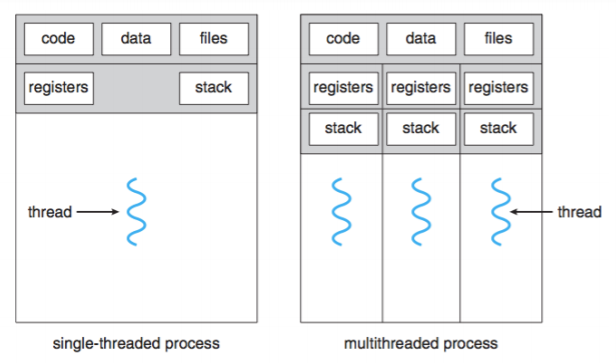
\includegraphics[width=12cm]{unit-14/figures/multithreading.png}
  \caption*{Single and multithreaded processes.}
\end{figure}

Most applications are multithreaded.
Applications are suitable for multithreading if they need several threads of control.
Examples include web browsers with separate threads for each tab, extension or native utility, as well as any GUI application, so that user events can still be handled while the main thread is performing a computation.

Multithreading is also used in systems that provide services, such as web servers and databases.
When the server receives a request, a new thread is created to service the request, while the main thread continues to listen for new requests.

Threads improve responsiveness, resource sharing and economy --- multithreading results in a smaller memory footprint and greater efficiency of switching between threads.
Threads also improve scalability by enabling the use of parallel processing in multithreaded processors.
They also reduce program complexity by breaking problems into smaller, independent tasks that can execute in parallel.

A system is parallel if it can perform more than one task simultaneously.
A concurrent system supports more than one task by allowing each task to make progress.
Concurrency can be achieved without parallelism.

\subsection{Multicore Systems and Multithreading}

Amdahl's law describes the ratio of the performance of a process running on a single processor to its performance running on multiple processors in terms of the proportion \(f\) of its code that is parallelisable and the number \(N\) of parallel processors.
This ratio is known as `speedup'.
The difference \(\left(1 - f\right)\) is the proportion of the code that is inherently serial.

\begin{equation*}
  \text{speedup} = \frac{\text{time to execute on a single processor}}{\text{time to execute on \(N\) parallel processors}} = \frac{1}{\left(1 - f\right) + \frac{f}{N}}
\end{equation*}

Even a small amount of serial code has a noticeable impact on the overall performance.
There are also overheads to parallelism that are not considered by Amdahl's law.
Latency is introduced by memory access and cache loading, for example.

Parallel programming introduces a number of challenges.
Pressure is placed on system designers to make better use of multiple cores and to write scheduling algorithms that allow parallel execution.
It is difficult both to modify existing programs and to design new programs to make use of multithreading.
This involves identifying tasks that can be divided into separate, concurrent and, ideally, independent tasks, balancing tasks to achieve efficiency, splitting data, and identifying data dependencies.
It is also difficult to test and debug parallel execution since it is non-deterministic.

\subsection{Multithreading Models}

Threads are used through a thread library that exists on the OS or virtual machine.
Operating systems and programming languages provide APIs for creating and managing threads.

Threads may exist at either the user or kernel levels.
User threads are managed above the kernel.
Kernel threads are managed by the OS directly.
Threads can be mapped to processes using three models.

\subsubsection{Many-to-One Model}

The many-to-one model maps many user-level threads to one kernel thread.
Thread management is handled by the thread library in user space, so it is efficient.
However, only one thread can access the kernel at a time since a system call blocks other threads.
This model lacks parallelism on multicore systems and is, therefore, not widely used.

\subsubsection{One-to-One Model}

The one-to-one model maps each user thread to a kernel thread.
This overcomes the issue of blocking, and improves concurrency and parallelism.
However, for each user thread, there must be a kernel thread.

\subsubsection{Many-to-Many Model}

A software developer can create as many user threads as necessary in a thread pool.
Corresponding kernel threads can run in parallel on a multiprocessor.
If a thread blocks, the kernel can schedule another thread for execution.

\subsection{Thread Interference and Memory Consistency}

Threads communicate by sharing data.
If multiple threads reference the same object, thread interference can occur.
This happens when two functions operating on the same data interleave.
This is unpredictable and difficult to debug.

Memory consistency errors occur when different threads have inconsistent views of the same data.
This can be solved through synchronisation, which creates a happens-before relationship between methods and statements.
This guarantees that memory written by one statement is visible to another.

Two invocations of a synchronised method on the same object cannot be interleaved.
All other threads are blocked until the synchronised thread is complete.
When a synchronised method exits, it automatically establishes a happens-before relationship with any subsequent invocation of a synchronised method on the same object.

Synchronisation is based on intrinsic locks.
These enforce exclusive access and establish happens-before relationships.
Threads must acquire locks before they can do anything.


\section{Deadlocks}
\subsection{Reusable and Consumable Resources}

A reusable resource is used by only one process at a time and is not depleted by that use.
Reusable resources include processors, I/O channels, main and secondary memory, devices, and data structures such as files, databases and semaphores.
Processes obtain reusable resources and later release them for use by other processes.
A deadlock may occur if each process holds one such resource and requests another.

A consumable resource is created (or produced) and later destroyed (or consumed).
Consumable resources include interrupts, signals, messages and information in I/O buffers.
A deadlock may occur if two processes request information from each other at the same time.
Neither can send the required information because both are waiting for a response.

\subsection{Deadlock Conditions}

A deadlock is a permanent blocking of a set of processes competing for resources.
It is a circular resource conflict between a set of processes that occurs when each process currently holds a resource requested by another process and, therefore, each process is also waiting for another process to release its resource.

There exist four conditions that lead to a deadlock.
The first three are preconditions that, when all hold true, may lead to a deadlock.
If the forth condition occurs in addition to the first three, it is inevitable that a deadlock shall occur.

\begin{enumerate}
  \item Mutual exclusion --- only one process may use a resource at a time
  \item Hold-and-wait --- a process can hold a resource while it is waiting for other resources to become available
  \item No preemption --- processes cannot be interrupted to free their resources by force
  \item Circular wait --- processes wait for each other to release resources they wish to acquire, leading to a closed chain of processes
\end{enumerate}

A deadlock occurs when a circular wait occurs and cannot be resolved.
A circular wait cannot be resolved if the three preconditions are true.
Thus, if the first three conditions occur, there is a possibility of a deadlock, and if all four conditions occur there is an inevitable deadlock.

\subsection{Resource Allocation Graphs}

A resource allocation graph is a directed graph that depicts the state of a system of resources and processes.

\begin{figure}[htp]
  \centering
  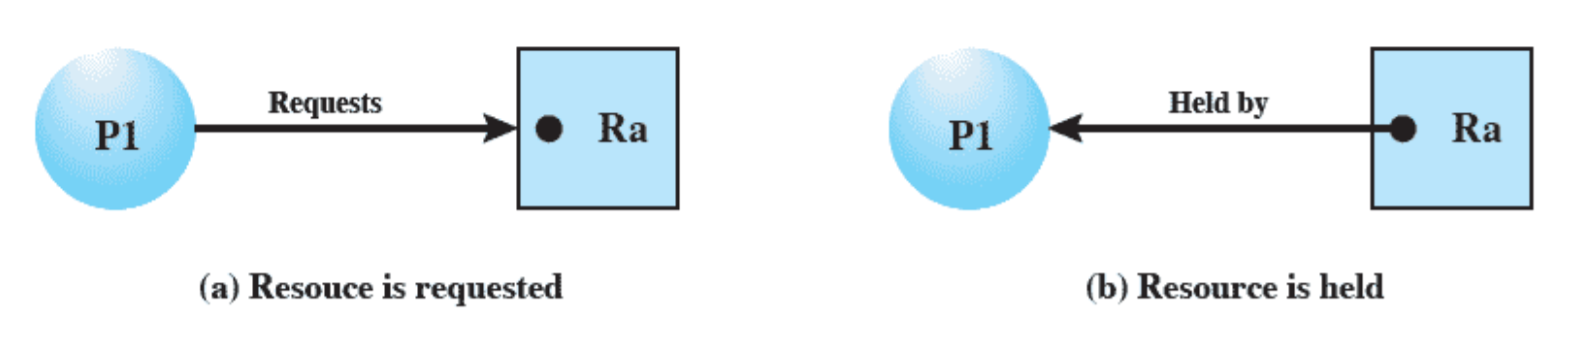
\includegraphics[width=15cm]{unit-15/figures/resource-graph-1.png}
  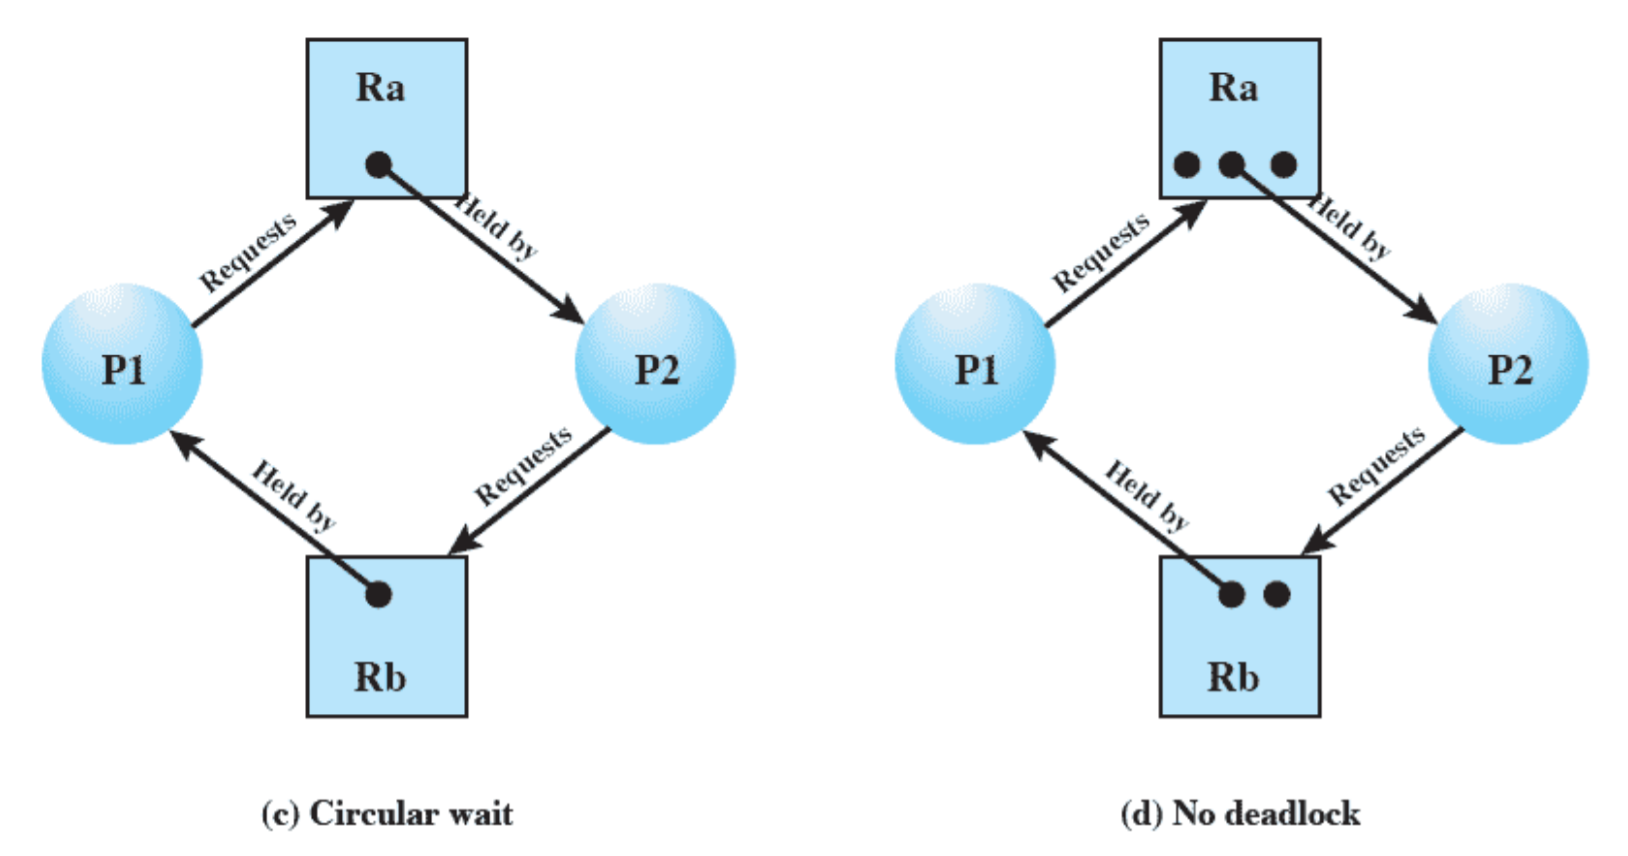
\includegraphics[width=15cm]{unit-15/figures/resource-graph-2.png}
\end{figure}

\subsection{Deadlock Handling}

Deadlocks can be handled through three methods.

\begin{itemize}
  \item Deadlock prevention
  \begin{itemize}
    \item Avoid at least one of the four deadlock conditions
  \end{itemize}
  \item Deadlock avoidance
  \begin{itemize}
    \item Requests for resources whose reservation may lead to deadlock are not granted
  \end{itemize}
  \item Deadlock detection and recovery
  \begin{itemize}
    \item No restriction on resource allocation
    \item Periodic check for deadlocks
    \item When a deadlock is detected, recovery mechanisms are employed
  \end{itemize}
\end{itemize}

\subsection{Deadlock Prevention}

In a deadlock prevention system, the OS is designed to prevent deadlocks from occurring.
The avoidance of the three preconditions is known as `indirect deadlock prevention'.
The avoidance of the final condition is known as `direct deadlock prevention'.

\subsubsection{Mutual Exclusion Prevention}

The mutual exclusion precondition cannot be avoided, as a lack of mutual exclusion may lead to race conditions.

\subsubsection{Hold-and-Wait Prevention}

The hold-and-wait precondition may be avoided by preallocating all required resources in advance and blocking a process until all its resources become available.
This results in long delays for processes, as well as low concurrency and inefficient utilisation of resources.
It is also difficult to achieve since a process may not know in advance what resources it may require.

\subsubsection{No Preemption Prevention}

The avoidance of this condition may be achieved in different ways.
If a process is holding a resource and is denied a request for another resource, it may be preempted.
Alternatively, the process holding the other resource may be preempted.
These methods are only possible if the state of the resources can be saved and restored so that the preempted process may resume execution.

\subsubsection{Circular Wait Prevention}

One method of direct deadlock prevention is to associate an index to each resource.
A process that requires multiple resources must acquire them in ascending index order.
For example, if two processes are competing for resource~1 and resource~2, the first process will acquire resource~1 and is free to acquire resource~2, since the second process cannot acquire either; the second process cannot acquire resource~2 before resource~1, and cannot access resource~1 because it is locked.
This method of resource ordering to prevent circular waits is usually inefficient because processes that use common resources are forced to execute in series rather than parallel.

\subsection{Deadlock Avoidance}

In a deadlock avoidance system, the decision of whether to grant a resource allocation is made dynamically depending on whether it is at all possible that such a request may lead to a deadlock.
This method requires knowledge of future resource requests.
The three preconditions are not avoided.
Instead, intelligent decisions are made when allocating resources.

\begin{itemize}
  \item Process initiation denial --- do not start a process if its demands may lead to deadlock
  \item Resource allocation denial --- do not grant an incremental resource request to a process if the allocation may lead to deadlock
\end{itemize}

\subsubsection{The Resource Matrix System}

Resources and process that require them can be represented using vectors and matrices.
The system resource vector \( \mathbf{r} \) is a vector of the total number of instances of each resource in the system.

\begin{equation*}
  \mathbf{r} = \left[ r_1, r_2, \ldots, r_n \right]
\end{equation*}

The available resource vector \( \mathbf{v} \) is a vector of all available resources (resources that are not in use).

\begin{equation*}
  \mathbf{v} = \left[ v_1, v_2, \ldots, v_n \right]
\end{equation*}

The claim matrix \( \mathbf{C} \) represents the resource requirement of each process.
An element \( c_{pr} \) is the number of instances of resource \( r \) required by process \( p \).
Each row \( \mathbf{c}_p \) represents the total resource claim of process \( p \).

\begin{equation*}
  \mathbf{C} = \begin{bmatrix}
    c_{11} & c_{12} & \ldots & c_{1n} \\
    c_{21} & c_{22} & \ldots & c_{2n} \\
    \vdots & \vdots & \ddots & \vdots \\
    c_{m1} & c_{m2} & \ldots & c_{mn} \\
  \end{bmatrix}
\end{equation*}

The allocation matrix \( \mathbf{A} \) represents the resource allocation of each process.
An element \( a_{pr} \) is the number of instances of resource \( r \) allocated to process \( p \).
Each row \( \mathbf{a}_p \) represents the total resource allocation of process \( p \).

\begin{equation*}
  \mathbf{A} = \begin{bmatrix}
    a_{11} & a_{12} & \ldots & a_{1n} \\
    a_{21} & a_{22} & \ldots & a_{2n} \\
    \vdots & \vdots & \ddots & \vdots \\
    a_{m1} & a_{m2} & \ldots & a_{mn} \\
  \end{bmatrix}
\end{equation*}

All the resources in the system are either available or allocated.

\begin{equation*}
  r_r = v_r + \sum_p a_{pr} \quad \forall r
\end{equation*}

No process may claim more instances of a resource than exist in the system.

\begin{equation*}
  c_{pr} \le r_r \quad \forall p, r
\end{equation*}

No process is allocated more instances of a resource than it claims.

\begin{equation*}
  a_{pr} \le c_{pr} \quad \forall p, r
\end{equation*}

\subsubsection{Process Initiation Denial}

A new process \( \left( n + 1 \right) \) is initiated only if the sum of claims of the new process and all the currently running processes can be met by the system.

\begin{equation*}
  r_r \ge c_{\left( n + 1 \right) r} + \sum_{p = 1}^n c_{pr} \quad \forall r
\end{equation*}

This deadlock avoidance scheme assumes the worst possible scenario --- that all processes will demand their resources at the same time.

\subsubsection{Resource Allocation Denial}

Resource allocation denial is achieved through the `banker's algorithm'.
A process is only allocated a resource if the system will remain in a safe state --- a state in which there exists at least one sequence of resource allocations that does not result in a deadlock.

A system is in a safe state if any of the participating processes can run to completion with the resources available, i.e.\ the difference between the requirement and allocation of any process can be met with the resources available.

\begin{equation*}
  c_{pr} - a_{pr} \le v_r \quad \forall r
\end{equation*}

Deadlock avoidance is less restrictive than deadlock prevention since resources can be allocated out of order.
However, the maximum resource requirement of all processes must be known in advance, processes under consideration must be independent (without synchronisation), the number of instances of resources in the system must remain constant, and no processes may exit whilst holding resources.

\subsection{Deadlock Detection and Recovery}

The algorithm for deadlock detection is as follows.
\begin{enumerate}
  \item Unmark (assume deadlocked, mark with T) all processes and define a matrix \( \mathbf{Q} \) that represents the future requests of each process.
  \item Mark (assume complete, mark with F) all processes that have zero resources allocated to them.
  These processes have reached completion.
  \item Initialise a temporary vector \( \mathbf{w} \) equal to the available resource vector \( \mathbf{v} \).
  \item Find a process \( p \) that is unmarked (assumed deadlocked, marked with T) such that the future requests of the process can be met by the currently available resources (\( q_{pr} \le w_r \quad \forall r \)).
  \item If such a process is found, update each resource \( r \) in the currently available resources \( \mathbf{w} \) as if the resources allocated to the process have been freed (\( w_r \mapsto w_r + a_{pr} \quad \forall r \)), and mark (assume complete, mark with F) process \( p \).
  Repeat from step \num{4}.
  \item If no such process is found, continue to step \num{7}.
  \item All unmarked (marked with T) processes are deadlocked processes.
\end{enumerate}

If a deadlock is detected, there are several methods to recover from it.
\begin{itemize}
  \item Abort all deadlocked processes.
  \item Roll back each deadlocked process to a previous state and resume.
  \item Abort deadlocked processes one by one until the deadlock disappears.
  \item Release the resources by force via preemption until the deadlock disappears.
\end{itemize}

The order of preemption or abortion should be based on some criteria, such as increasing order of resource usage.

\subsection{Integrated Deadlock Strategy}

An integrated deadlock strategy is a combination of deadlock handling approaches.
Resources can be grouped into resources classes.
For example,
\begin{itemize}
  \item swappable space --- blocks of memory on secondary storage used for swapping processes,
  \item process resources --- assignable devices or files, and
  \item main memory --- assignable to processes in pages or segments.
\end{itemize}

Different deadlock handling strategies can be applied to each resource class.
\begin{itemize}
  \item Swappable space --- deadlock prevention (all required resources are allocated at once, maximum storage requirements are known)
  \item Process resources --- deadlock avoidance (processes declare ahead of time the resources they will require) or deadlock prevention (resource ordering)
  \item Main memory --- deadlock prevention by preemption
\end{itemize}

\begin{table}[htp]
  \centering
  \caption*{Summary of deadlock handling approaches.}
  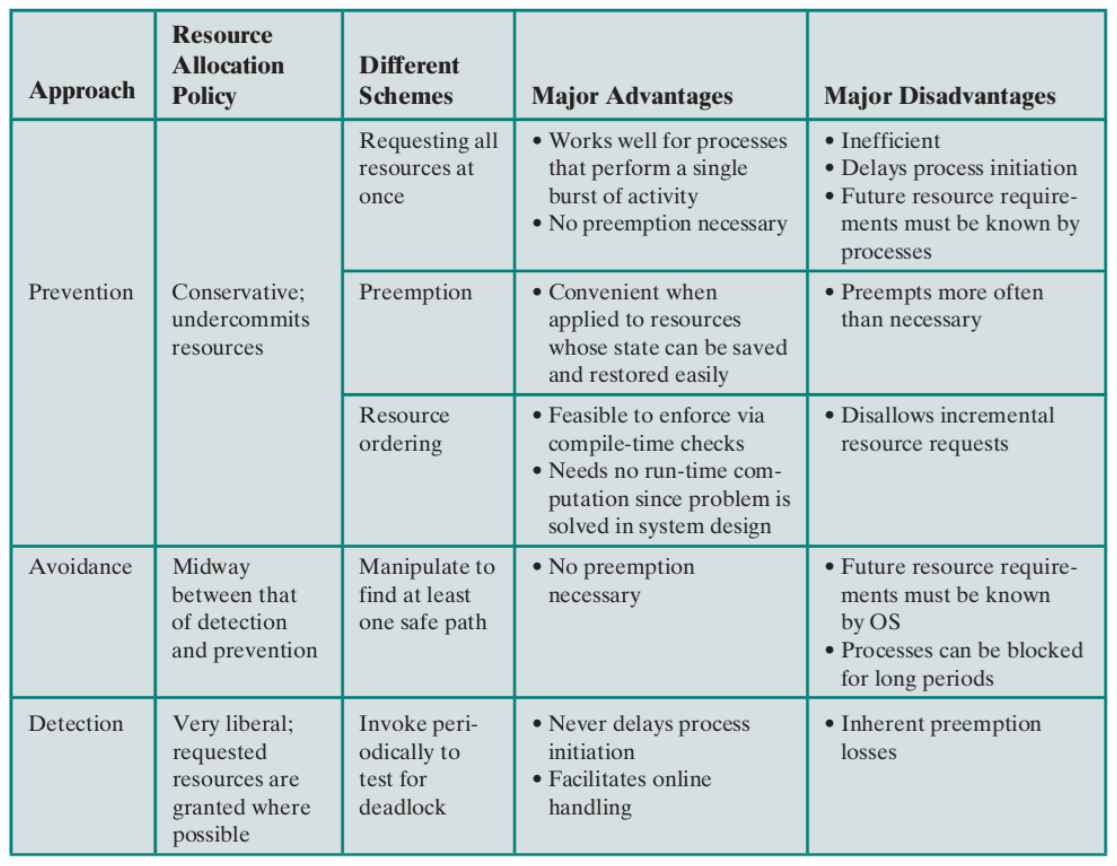
\includegraphics[width=15cm]{unit-15/figures/deadlock-summary.png}
\end{table}


\section{Introduction to Networks}
\subsection{The Internet}

The Internet consists of billions of connected computing devices.
End systems are also known as `hosts' and run network applications.
Computers are connected via communication links, which can be fibre optic, copper, radio or satellite.
End systems and different networks are connected to routers and packet switches that forward chunks of data known as `packets'.

The Internet is a network of networks and interconnected Internet service providers (ISPs).
The sending and receiving of messages is controlled by protocols such as TCP, IP, HTTP, Skype and 802.11.
A set of standards exists to help manage the Internet.
Proposals for standards and protocols are published as requests for comments (RFCs), which are made available to key stakeholders to be reviewed and standardised.
The Internet Engineering Taskforce (IETF) is the governing body that oversees the development of the Internet.

The Internet is also an infrastructure that provides services to applications.
These services and applications include web, VoIP, email, games, e-commerce and social networks.
It also provides a programming interface to applications.
Web hooks allow applications to connect to the Internet.

Residential, institutional and mobile access networks each have end systems connected to an edge router.
The bandwidth of a connection is affected by the hardware and connection used.
Radio links are shared, whereas an Ethernet cable is dedicated.

Client and server hosts, and servers in data centres form the network edge.
Access networks are the communication links between devices.
These may be wired or wireless.
The interconnected routers that connect the access networks are known as the `network core'.

Hosts break application messages into smaller chunks known as `packets' and transmit them to the access network.
The speed at which the packet is transmitted to the access network is the link transmission rate, which is also known as `link capacity' or `link bandwidth'.
The packet transmission delay when a packet of length \( L \)~bits is transmitted into a link with transmission rate \( R \)~bits per second is \( \frac{L}{R} \)~seconds.

The network core forwards packets from one router to the next across links that form a path between source and destination.
Each packet is transmitted at full link capacity.
Routing algorithms in the network core determine the source to destination route taken by packets.
Routers forward packets from their input to their appropriate output.

\subsection{Distributed Systems}

A distributed system is one in which hardware or software components located at networked computers communicate and coordinate their actions by only passing messages.
Distributed networks allow for high concurrency.
There is no global notion of the correct time in a distributed network; there is only relative time between computers.
Each component in a network may fail independently.
The failure of one component does not affect the other components.

\subsection{Internet, Intranet and Firewalls}

The Internet is a distributed system that enables users all over the world to make use of its services.
Some highly connected links in the Internet are known as backbones.
These have high link capacity and can be connected via satellite link.

An intranet is part of the Internet that is separately administered and uses a firewall to enforce its own local security policies.
Users in an intranet share data by means of file services.

A firewall is a network security system that monitors and controls incoming and outgoing network traffic according to predetermined security rules.
A firewall establishes a barrier between a trusted internal network and an untrusted external network, such as the Internet.
Firewalls may be network-based or host-based, including network-layer or packet filters and application-layer firewalls.

\subsection{Network Principles}

Networking is concerned with sending messages over a carrier.
\begin{itemize}
  \item Latency is the term given to any kind of delay that occurs during data communication over a network.
  \item Bandwidth is the transmission capacity of a computer network or telecommunication system.
  \item Speed is the rate at which data is able to move.
\end{itemize}

A logical unit of data transmitted via a network is known as a message.
A message of arbitrary length is divided into packets before transmission.
A packet is a bit stream of restricted length.
It includes not only the data, but also relevant addressing information.

\subsection{Switching Schemes}

A network is a set of nodes connected by circuits.
In order to transmit information between two nodes, a switching scheme is required.
\begin{itemize}
  \item Broadcast --- no switching, data is transmitted throughout the network
  \item Circuit switching --- source and destination are connected through a switch at an exchange
  \item Packet switching --- a store-and-forward network with a computer at each end
\end{itemize}

\subsubsection{Circuit Switching}

End-to-end resources are allocated to create a reserved connection between source and destination.
The resources are dedicated; there is no sharing.
Full bandwidth circuit-like performance is guaranteed.
Circuit segments remain idle if not used for a connection.
This transmission scheme is traditionally used in telephone networks.

\subsubsection{Packet Switching}

Packet switching is a store-and-forward transmission scheme that allows more users to use the network.
Packets are transmitted to a router, where they are stored in a queue, waiting for an output link.
The entire packet must arrive at the router before it can be transmitted through the next link.

The delay for transmission of an \( L \)~bit packet through an \( R \)~bits per second link is \( \frac{L}{R} \)~seconds.
This is the `one-hop transmission delay'.
Assuming no propagation delay, the end-to-end delay for transmission from source to destination through one router is \( 2 \frac{L}{R} \).
In general, the delay is \( N \frac{L}{R} \), where \( N \) is the number of links and, therefore, \( N - 1 \) is the number of routers.

If the arrival rate to a router exceeds its transmission rate for a period of time, the packets will queue, waiting to be transmitted through a link.
Additionally, packets can be dropped (lost) if the memory (buffer) is filled.

\subsection{Internet Structure (Network of Networks)}

End systems connect to the Internet via access ISPs.
These may be residential, company or university ISPs.
In turn, access ISPs must be interconnected so that any two hosts can communicate.
The resulting network is very complex.
Its evolution has been driven by economics and national policies.

Connecting each access ISP to every other access ISP is not feasible.
This would require \( \function{O}{n^2} \) connections.
An alternative is to connect each access ISP to a global ISP\@.
There would be an economic agreement between customer and provider ISPs.
However, if one global ISP is a viable business, there will exist competitors, which must in turn be interconnected.

Such global ISPs are connected to each other through Internet exchange points (IXPs) or peering links.
Regional networks also exist to connect groups of access networks to global ISPs.
Large Internet companies, such as Google and Microsoft, run their own content delivery networks to bypass connections and provide services and content closer to end systems.

The result is small number of well-connected large networks.
These are `Tier~1' commercial ISPs that offer national and international coverage, and private content delivery networks that connect data centres to the Internet to bypass Tier~1 and regional ISPs.

\subsection{Packet Loss and Delays}

When the arrival rate of packets at a router exceeds the output link capacity, the packets wait in a buffer queue for transmission.
A packet is dropped (lost) if there is no available buffer space in the queue when it arrives.
A lost packet may be retransmitted by the previous node, the end system source or not at all.
Nodal delay \( d_{\text{nodal}} \) is the delay of packets at a node in a network.

\begin{equation*}
  d_{\text{nodal}} = d_{\text{proc}} + d_{\text{queue}} + d_{\text{trans}} + d_{\text{prop}}
\end{equation*}

\begin{itemize}
  \item Nodal processing delay (\( d_{\text{proc}} \))
  \begin{itemize}
    \item Time spent checking bit errors and determining output link
    \item Typically less than a millisecond
  \end{itemize}
  \item Queueing delay (\( d_{\text{queue}} \))
  \begin{itemize}
    \item Time spent waiting at output link for transmission
    \item Dependent upon congestion level at link/router
  \end{itemize}
  \item Transmission delay (\( d_{\text{trans}} \))
  \begin{itemize}
    \item Time spent placing packet onto output link
    \item For a packet of length \(L\)~\si{\bit} and link of bandwidth \(R\)~\si{\bit\per\second}, \( d_{\text{trans}} = \frac{L}{R} \)~\si{\second}
  \end{itemize}
  \item Propagation delay (\( d_{\text{prop}} \))
  \begin{itemize}
    \item Time spent travelling through output link to next node
    \item For a link of length \(d\)~\si{\metre} and a propagation speed through the link medium of \(s\)~\si{\metre\per\second}, \( d_{\text{prop}} = \frac{d}{s} \)~\si{\second}
  \end{itemize}
\end{itemize}

Throughput is the rate at which bits are transferred between sender and receiver.
Throughput can be measured as instantaneous throughput at a specific point in time or average throughput over a longer period of time.
The average end-to-end throughput is determined by the link with the lowest capacity.
A link on an end-to-end path that constrains the throughput is known as a `bottleneck link'.

\subsection{Protocols}

Network protocols define a set of guidelines that allow network devices to communicate effectively.
A protocol defines the sequence of messages that should be exchanged and the format of the data in the messages.
Protocols are implemented by pairs of software modules in the sending and receiving systems.

A transport protocol transmits a message from a sender to a receiver.
A process that wishes to send a message passes it to the transport protocol module.
The software divides the message into packets, which are then transmitted using the network protocol.
Inverse operations are performed by the receiver to reconstruct the message.

\begin{figure}[htp]
  \centering
  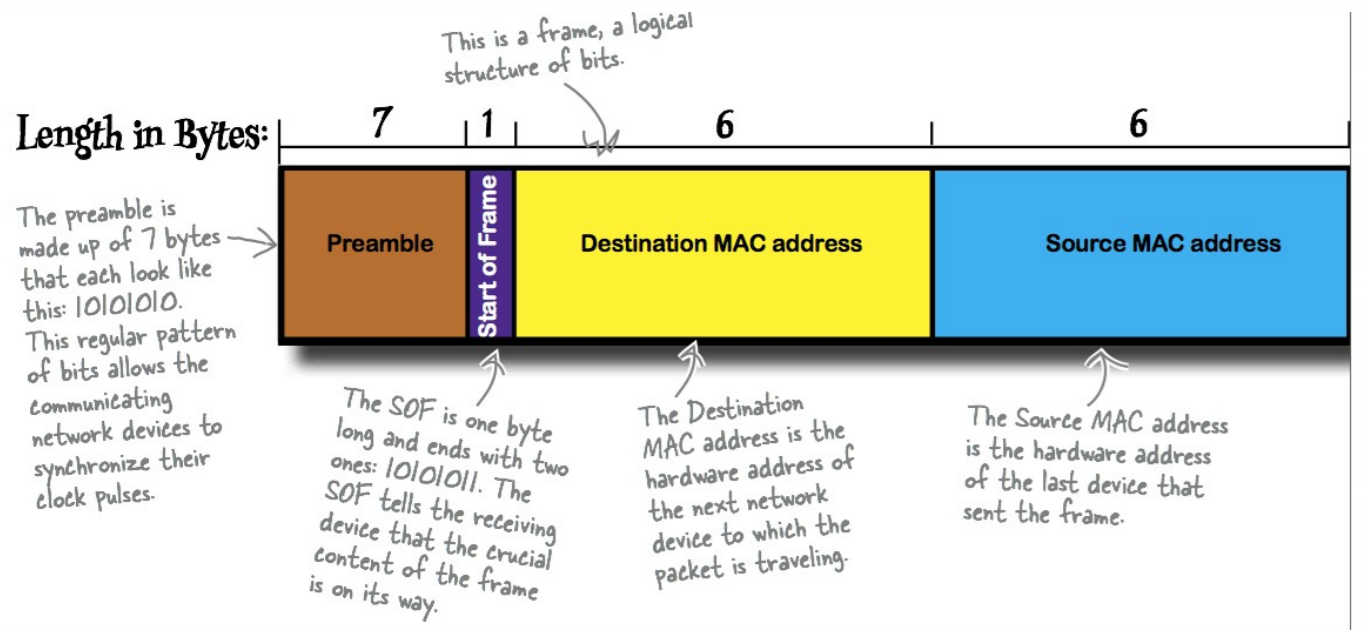
\includegraphics[width=15cm]{unit-16/figures/frame-part-1.png}
  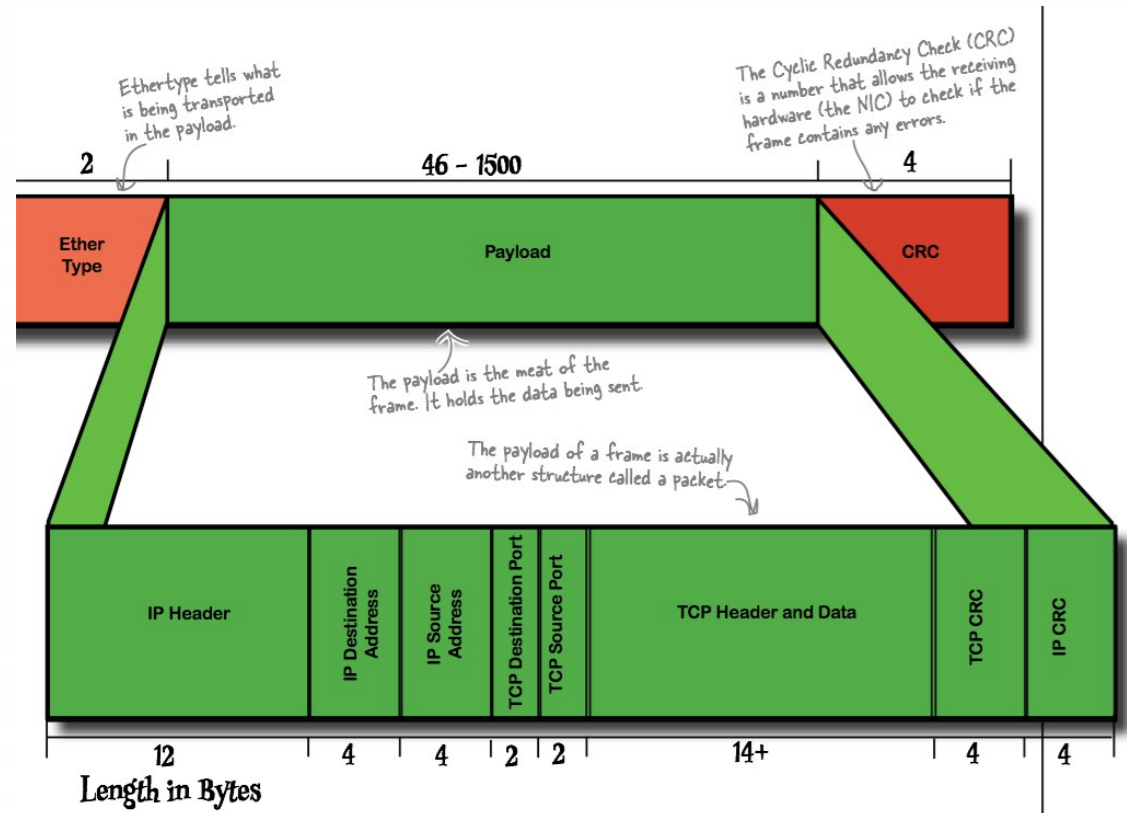
\includegraphics[width=15cm]{unit-16/figures/frame-part-2.png}
  \caption*{The structure of a packet frame.}
\end{figure}

\subsection{Protocol Layers and Encapsulation}

Network software is arranged in a hierarchy of layers, in which each layer presents an interface to the layer above.
Each layer accepts an item of data in a specified format from the layer above.
It applies a transformation to the data in order to encapsulate it.
The data is passed to the layer below.
Layers communicate with those directly above and below through procedure calls.
Every computer in a network must have these layers.

A complete set of protocol layers is known as a `protocol suite' or `protocol stack'.
Each layer adds a header to the data before it is sent.

\subsection{Open Systems Interconnection (OSI) Model}

The Open Systems Interconnection (OSI) model is a conceptual protocol stack model.
Its layers from highest to lowest are
\begin{itemize}
  \item application,
  \item presentation,
  \item session,
  \item transport,
  \item network,
  \item (data) link, and
  \item physical.
\end{itemize}

Data are passed down through the layers in the source end system and across the network via physical connections.
Switches and routers use the data link and network layers to route the data through the network.
When the data arrive at the end system, they are passed up through the layers and are reconstructed.

\begin{table}[htp]
  \centering
  \caption*{The layers of the OSI model.}
  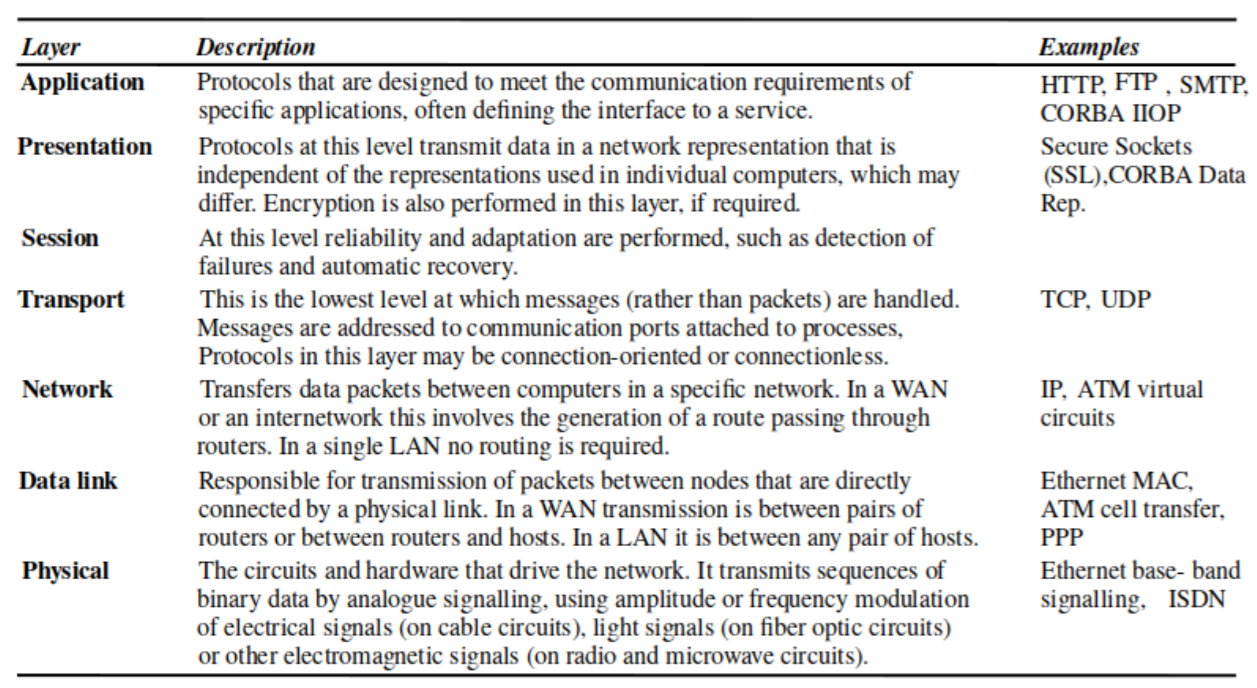
\includegraphics[width=15cm]{unit-16/figures/layer-summary.png}
\end{table}

Protocol layering simplifies and generalises the software interfaces that access communication services.
However, they reduce the performance of the network.
A total of \(N\) protocol layers results in \(N\) control transfers for each message at an end system, and \(N\) copies of the data due to encapsulation.
Thus, the data transfer rate may be much slower than the available network bandwidth.

The five-layer protocol stack used by the Internet differs from the seven-layer OSI model.
Its layers from highest to lowest are
\begin{itemize}
  \item application,
  \item transport,
  \item network,
  \item link, and
  \item physical.
\end{itemize}
The application, presentation and session layers of the OSI model are not clearly distinguished in the Internet protocol stack, and are instead all part of a single application layer.
Applications are responsible for deciding how to handle these protocols.
The session layer is integrated with the transport layer.

\subsection{Large Messages and Message Consistency}

An Ethernet frame can only hold \SI{1500}{\byte} of data.
Messages larger than this limit must be broken into packets.
Message consistency and reliable data transfer are achieved by communicating via the Transmission Control Protocol (TCP).
If there are errors in the packets, the receiver notifies the sender, and those packets are sent again.
If the message is a single long packet, there may be issues due to poor connection.

Packets may not be received in the same order that they are sent.
Each packet contains a sequence number so that they can be reordered correctly.

\subsection{Ports and Addressing}

The responsibility of the transport layer is to provide a network-independent message transfer service between pairs of network ports.
The destination ports at a host computer are defined by software and are attached to processes.
Port~\num{25} is used for email.

The transport layer delivers messages to destinations specified by transport addresses.
A transport address comprises a network address and a port number.
In the Internet, every host system is assigned an Internet Protocol (IP) address that identifies it and the subnet to which it is connected.

\subsection{Datagram Packet Delivery}

In datagram packet delivery, it is the responsibility of the receiver to indicate if there is a problem with transmission.
The network retains no information after it has been delivered.
The sequence of packets may take different routes from host to destination, so they may arrive out of sequence.
Datagrams contain the full network addresses of the source and destination.
The network layer of the Internet uses datagram delivery.

A link-layer switch accesses the data link layer of a packet to determine the next link to which the packet must be sent.
A router is a three-layer switch.
It accesses the network layer of the packet in order to route the packet to the destination host.


\section{Application Layer}
\subsection{Principles of Network Applications}

Network applications run on different end systems and communicate over a network.
For example, a browser communicates with web server software.
There is no need to write network applications for network-core devices.
Applications run only on end systems.
This allows for rapid application development and propagation.
Network applications can follow either client-server or peer-to-peer (P2P) architecture.

\subsubsection{Client-Server Architecture}

In a client-server architecture, the server is an always-on host with a permanent IP address and data centres for scaling.
Clients communicate with the server, and may have intermittent connections and dynamic IP addresses.
Clients do not communicate with each other directly.

\subsubsection{Peer-to-Peer (P2P) Architecture}

In a peer-to-peer architecture, there is no always-on server.
Arbitrary end systems communicate directly.
Peers request and provide services from and to other peers.
Such an architecture is self-scalable; new peers bring additional service capacity as well as additional service demands.
Peers are intermittently connected and have dynamic IP addresses.
This requires a complex management of connections.

\subsubsection{Process Communication and Sockets}

A process is a program running within a host.
Within a host, two processes communicate using inter-process communication methods defined by the OS\@.
Two processes in different hosts must communicate by exchanging messages.
A client process is a process that initiates communication.
A server process is a process that waits to be contacted.
P2P applications use both client processes and server processes.

A process sends and receives messages to or from its socket.
A sending process relies on the transport infrastructure on the outside of its socket to deliver its message to the socket at the receiving process.

In order to receive messages, each process must have an identifier.
Every host has a unique \SI{32}{\bit} IP address.
The process identifier comprises the host IP address and the port number associated with the process on the host.
Example port numbers include \num{25} for mail servers and \num{80} for HTTP servers.

\subsection{Transport Services}

Network applications require different transport services.
\begin{itemize}
  \item Data integrity
  \begin{itemize}
    \item Some apps, such as file transfer and online transactions, require reliable data transfer.
    \item Other apps, such as audio streaming, can tolerate some loss.
  \end{itemize}
  \item Timing
  \begin{itemize}
    \item Some apps, such as Internet telephony and games, require low delay to be effective.
  \end{itemize}
  \item Throughput
  \begin{itemize}
    \item Some apps, such as multimedia streaming, require a minimum level of throughput to be effective.
    \item Other apps, known as `elastic apps', make use of whatever throughput they can get.
  \end{itemize}
  \item Security
  \begin{itemize}
    \item Some apps require encryption and other security services.
  \end{itemize}
\end{itemize}

\begin{table}[htp]
  \centering
  \caption*{Transport service requirements of common applications.}
  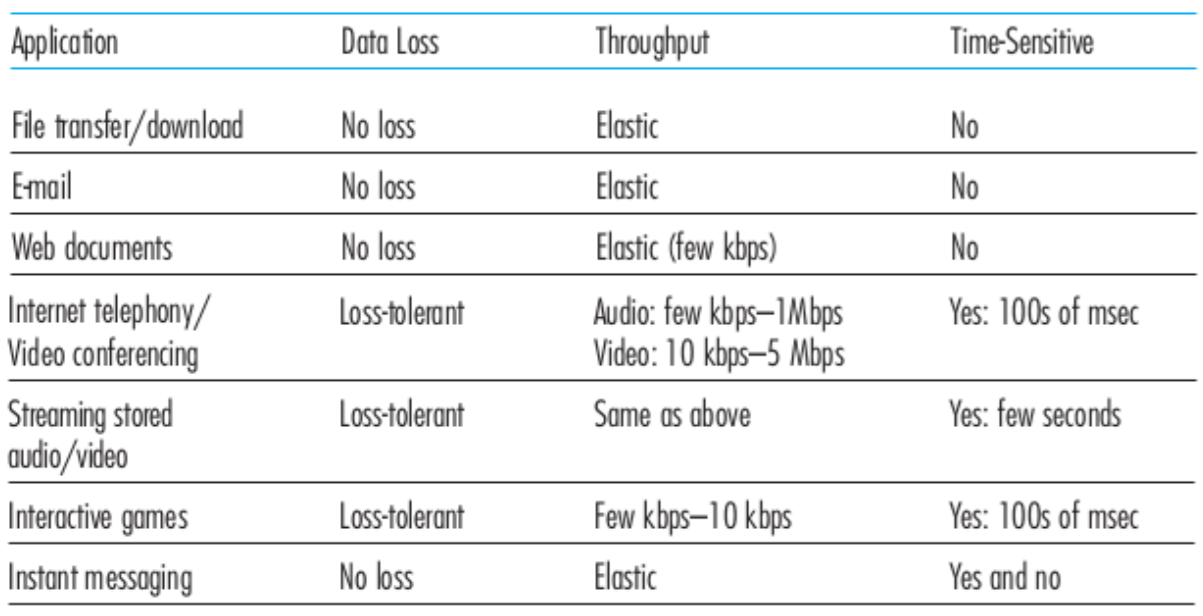
\includegraphics[width=12cm,height=4cm]{unit-17/figures/transport-service-requirements.png}
\end{table}

\subsubsection{Transmission Control Protocol (TCP)}

The Transmission Control Protocol (TCP) provides reliable transport between sending and receiving processes; the data received is identical to the data sent.
The protocol also provides flow control (so that the sender does not overwhelm the receiver) and congestion control (so that the sender is throttled when the network is overloaded).
The protocol does not provide guarantees for timing, minimum throughput or security --- these must be handled by the application layer.
TCP is a connection-oriented protocol; a connection must be set up between the client and the server before communication can occur.

\subsubsection{User Datagram Protocol (UDP)}

The User Datagram Protocol (UDP) provides unreliable data transfer between sending and receiving processes.
It does not provide reliability, flow control, congestion control, timing, throughput, security or connection setup.

UDP exists both because it is a very simple protocol to use and because it allows a lot more data to be transferred across a network than TCP\@.
Data integrity is sacrificed for greater throughput.
This is useful for Internet telephony applications.

\begin{table}[htp]
  \centering
  \caption*{Application and transport protocols of common applications.}
  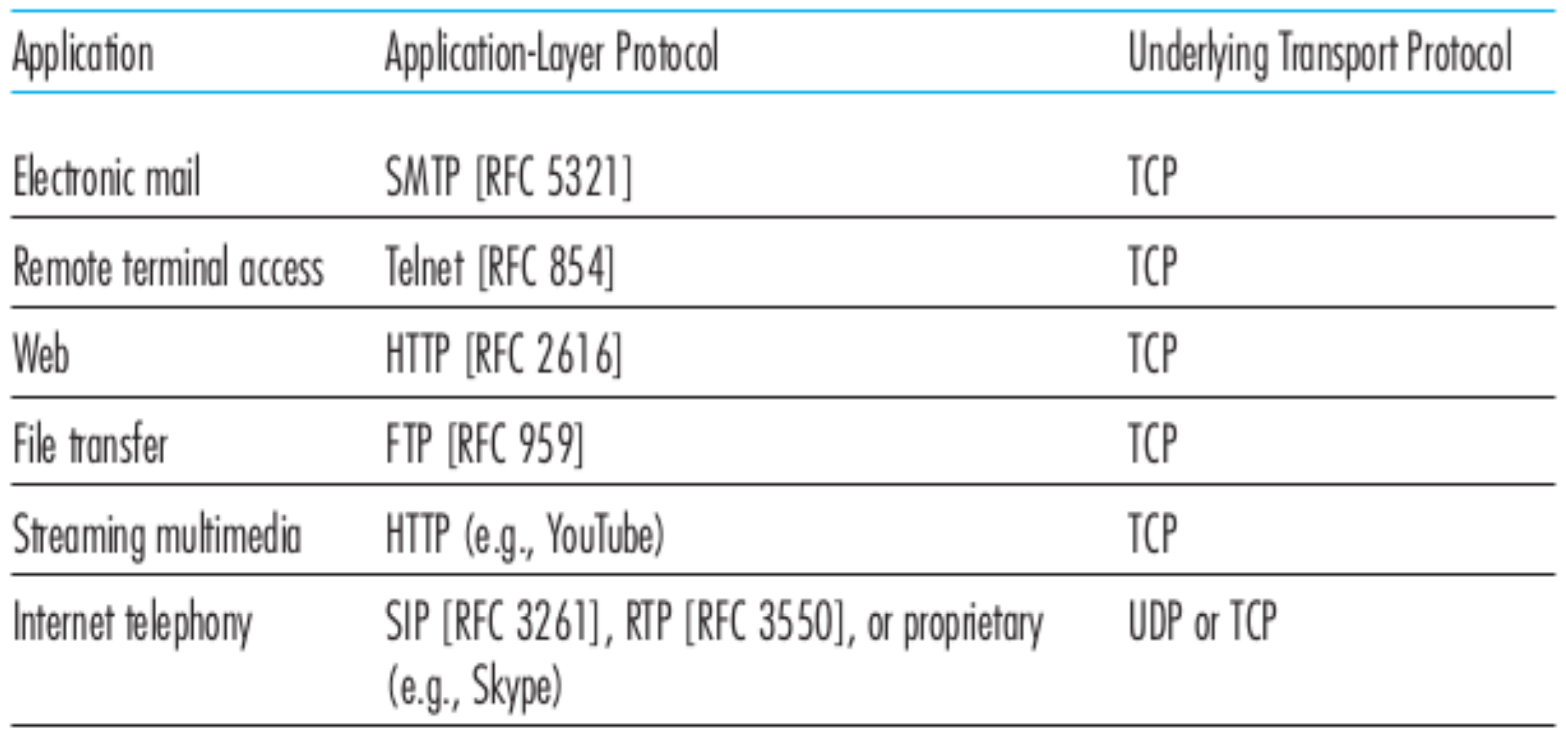
\includegraphics[width=12cm,height=4cm]{unit-17/figures/transport-protocols.png}
\end{table}

\subsection{Hypertext Transfer Protocol (HTTP)}

A web page consists of a base HTML file that may include several referenced objects, such as images, applets or media files.
Each object is addressable by a Uniform Resource Locator (URL), which consists of a host name and a path.

The Hypertext Transfer Protocol (HTTP) is the application layer protocol of the web.
The web uses a client-server architecture.
A web browser is a client that requests, receives and displays web objects.
The web server sends objects in response to requests.

HTTP uses the TCP protocol.
HTTP itself is a stateless protocol.
The server does not retain any information about past client requests.

\subsubsection{Non-Persistent HTTP}

\begin{enumerate}
  \item The HTTP client initiates a TCP connection to the HTTP server at the requested host address on port~\num{80}.
  \item The HTTP server accepts the connection and notifies the client.
  \item The HTTP client sends an HTTP request message (containing a URL to the requested object) through its TCP socket.
  \item The HTTP server receives the request message, forms a response message containing the requested object and sends its through its TCP socket.
  \item The HTTP waits until its message is received by the client, then closes the TCP connection.
  \item The HTTP client receives the response message and displays the HTML file.
  \item If object references are found in the HTML file, the above process is repeated for each object.
\end{enumerate}

The round-trip time (RTT) is the time it takes for a small packet to travel from the client to the server and back again.
The HTTP response time consists of one RTT to initiate the TCP connection, another RTT for the HTTP request to be sent and the HTTP response to start being received, and the file transmission time for the object being served.

\begin{equation*}
  \text{HTTP response time} = 2 \text{RTT} + \text{file transmission time}
\end{equation*}

\subsubsection{Persistent HTTP}

The use of non-persistent HTTP leads to a number of issues.
It takes two round-trips for each object and causes an OS overhead for each TCP connection.
Browsers often open parallel TCP connections to fetch referenced objects.

In persistent HTTP, the server leaves the connection open after sending a response.
Subsequent HTTP messages between the client and server are sent over an open connection.
This allows the client to send a request as soon as it encounters a referenced object.
This uses only one round-trip for each referenced object.

\subsubsection{HTTP Request Message}

HTTP messages are written in a human-readable ASCII format.
A request message begins with a request line, which contains the HTTP method (\texttt{GET}, \texttt{POST} or \texttt{HEAD}, for example).
The request line is followed by header lines.
The end of the header is indicated by a carriage return and line feed (CRLF) at the start of a line.

\begin{figure}[htp]
  \centering
  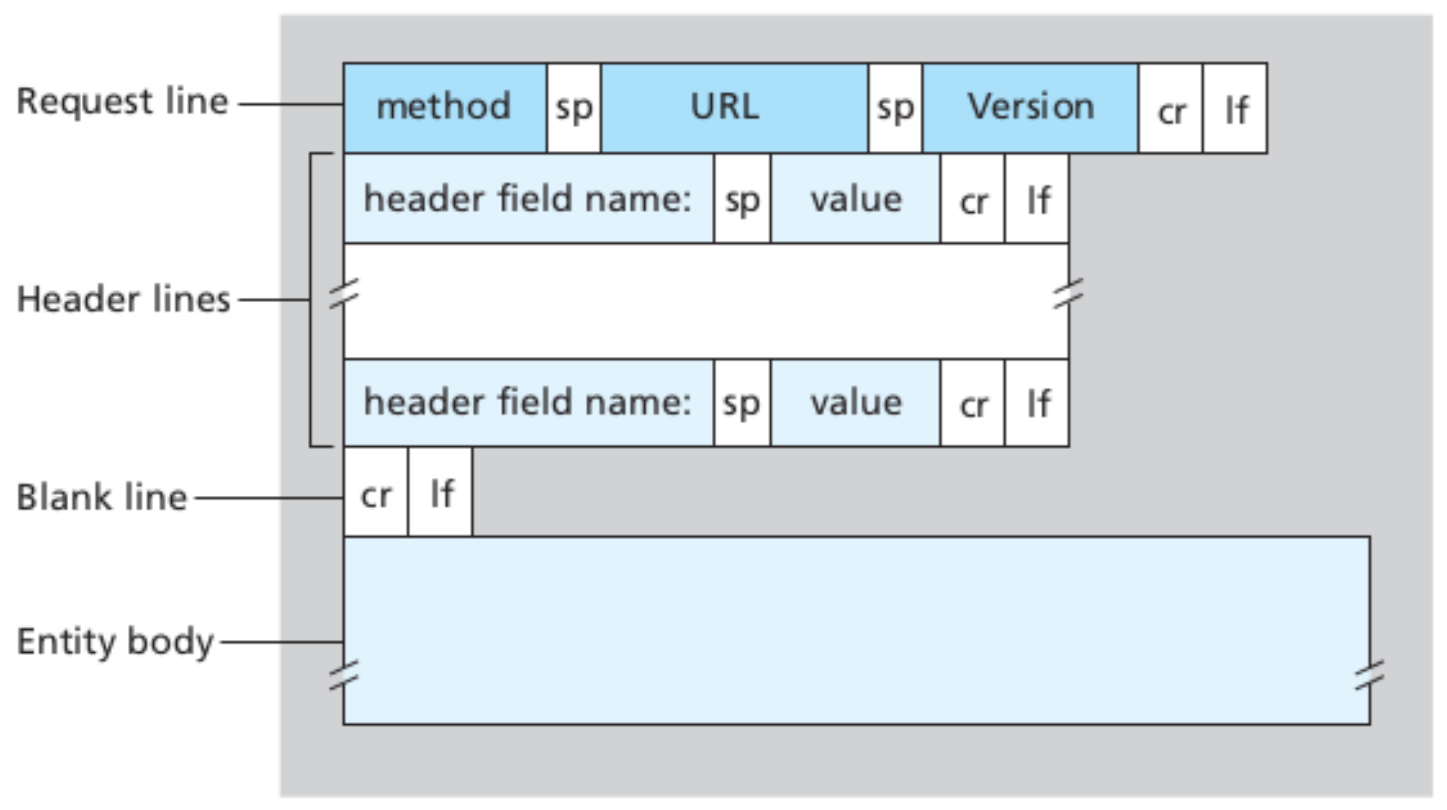
\includegraphics[width=12cm]{unit-17/figures/http-request.png}
  \caption*{General format of a HTTP request message.}
\end{figure}

\subsubsection{HTTP Response Message}

A response message begins with a status line, which contains the status code and status phrase.
Possible status codes and phrases include
\begin{itemize}
  \item 200 (OK) --- request succeeded, requested object contained in this message,
  \item 300 (Moved Permanently) --- requested object has moved to a new location specified in this message,
  \item 400 (Bad Request) --- request message not understood by server,
  \item 404 (Not Found) --- requested document not found on the server, and
  \item 505 (HTTP Version Not Supported).
\end{itemize}

The status line is followed by a header that ends with a CRLF at the start of a line.
The requested data follows the header.

\begin{figure}[htp]
  \centering
  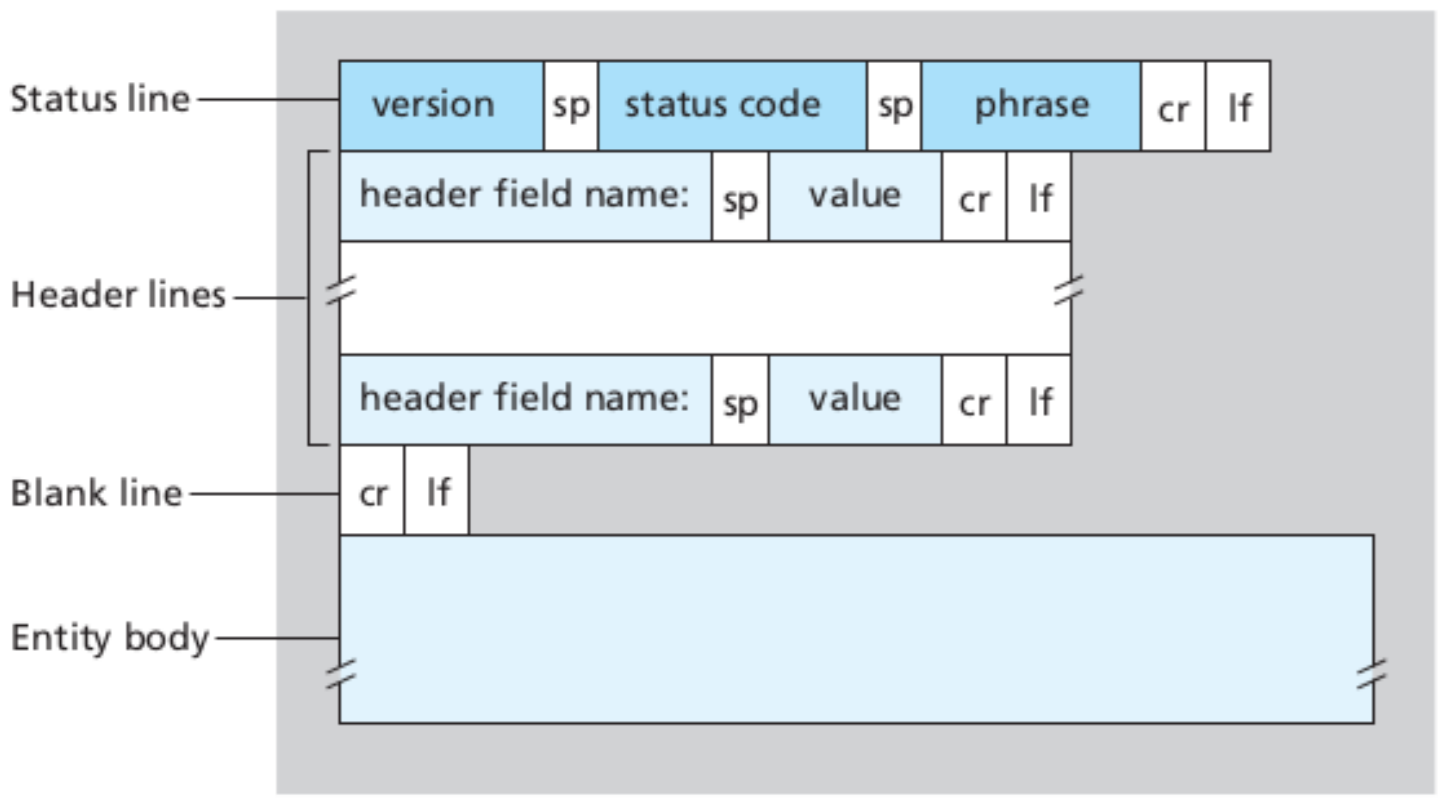
\includegraphics[width=12cm]{unit-17/figures/http-response.png}
  \caption*{General format of a HTTP response message.}
\end{figure}

\subsection{Simple Mail Transfer Protocol (SMTP)}

A user agent (UA) is an email client that is responsible for composing, editing and reading messages.
Incoming and outgoing messages are stored on a server.

A mail server contains mailboxes for each user that contain incoming messages and a message queue of outgoing messages.
The Simple Mail Transfer protocol (SMTP) is used to send email messages between mail servers.
A mail server takes on the role of client when it is sending emails, and the role of server when it is receiving emails.

SMTP uses TCP to reliably transfer emails directly from client to server at port~\num{25}.
An email transfer consists of three phases: handshake, transfer and closure.
SMTP uses a command and response interaction similar to that of HTTP\@.
Commands and responses are written in ASCII text and responses contain status codes and phrases.
SMTP commands include \texttt{HELO}, \texttt{MAIL FROM}, \texttt{RCPT TO}, \texttt{DATA} and \texttt{QUIT}.

SMTP uses persistent connections.
It requires that messages are composed in \SI{7}{\bit} ASCII\@.
The end of a message is indicated by a CRLF followed by a period and another CRLF\@.
Whilst HTTP uses a ``pull'' interaction, SMTP uses a ``push'' interaction.
In HTTP, each object is encapsulated in its own response message.
In SMTP, multiple objects can be sent in multipart messages.

\subsection{Mail Access Protocols}

Whilst SMTP is used for delivering and storing messages to the mail server of a receiver, a mail access protocol is used for retrieving messages from a server.
\begin{itemize}
  \item POP3 (Post Office Protocol Version 3) --- authorisation and download
  \item IMAP (Internet Mail Access Protocol) --- more features, including manipulation of a stored message on a server
  \item HTTP (Hypertext Transfer Protocol)
\end{itemize}

POP3 uses an authorisation phase, in which client issues \texttt{user} and \texttt{pass} commands to declare a username and password, and a transaction phase, in which the client issues \texttt{list}, \texttt{retr}, \texttt{dele} and \texttt{quit} commands to list message numbers, retrieve a message by number, delete a message by number and quit the server.

POP3 download-and-delete mode deletes messages from the server once they are downloaded to the client.
They cannot be downloaded again on another client.
POP3 download-and-keep mode allows copies of messages on multiple clients.
POP3 is stateless across sessions.

IMAP keeps all messages on the server and allows messages to be organised in folders.
IMAP retains the user state across sessions.
This includes the names of folders and the mappings of message identifiers to folder names.

\subsection{Domain Name System (DNS)}

Internet hosts and routers have \SI{32}{\bit} IP addresses used for addressing datagrams, and hostnames that are used by humans.
A Domain Name System (DNS) is a distributed database that maps hostnames to IP addresses.

A DNS provides
\begin{itemize}
  \item hostname to IP address translation,
  \item host aliasing (allows a host with a single canonical name to have multiple alias names),
  \item mail server aliasing, and
  \item load distribution (web servers are replicated such that many IP addresses correspond to one host name).
\end{itemize}

DNS is an application layer protocol used by hosts and name servers to communicate when resolving names.
DNS servers are end systems that exist at the network edge.
Lookup is performed as close as possible to the source host using a local DNS server.

A single centralised DNS does not exist as this would introduce a single point of failure.
It would also be impossible to implement as all Internet traffic would have to pass through a single server.
There would be long delays for end systems far from the server, and performing maintenance on the server would cause all Internet services to stop.

\subsubsection{The DNS Distibuted Hierarchical Database}

DNS is implemented using a hierarchy of many name servers.

\begin{figure}[htp]
  \centering
  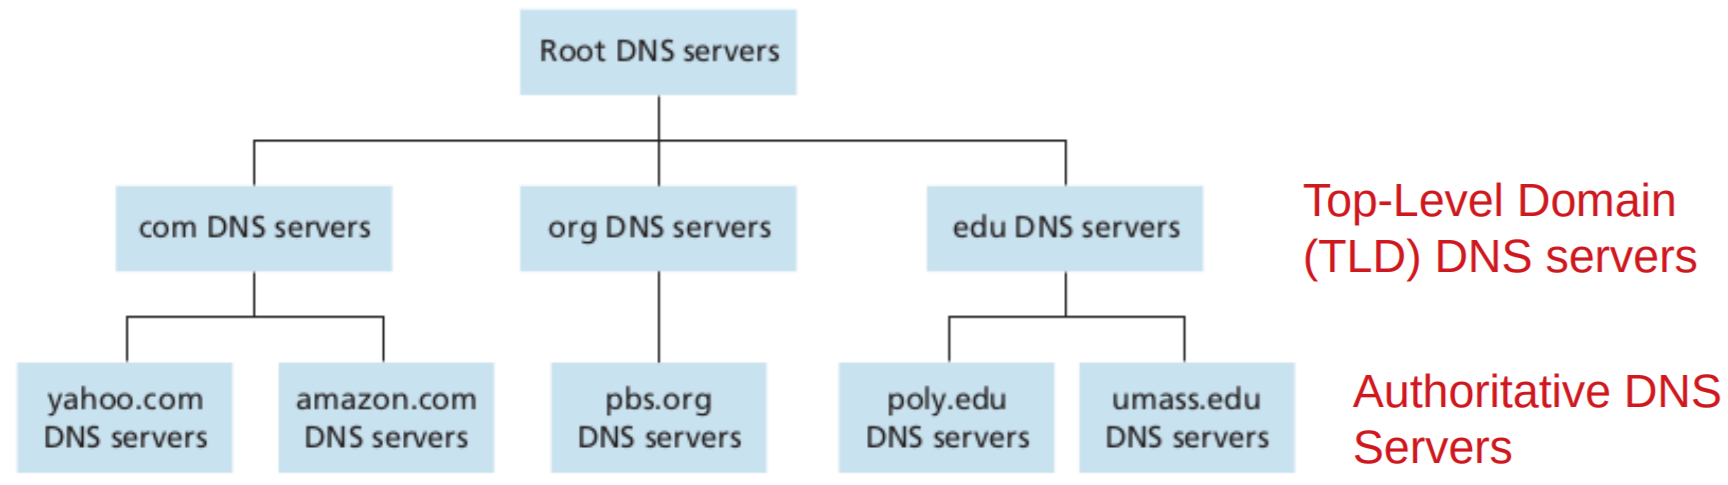
\includegraphics[width=15cm]{unit-17/figures/dns-hierarchy.png}
  \caption*{A portion of the hierarchy of DNS servers.}
\end{figure}

There are several root DNS servers worldwide.
Each is actually a network of replicated servers.
A top-level domain (TLD) server is responsible for \texttt{com}, \texttt{org}, \texttt{net}, \texttt{edu}, \texttt{gov} and all top-level country domains.
An authoritative server is a DNS server owned by an organisation.
It provides authoritative hostname to IP mappings for the named hosts of the organisation.
These can be maintained by the organisation itself or a service provider on its behalf.

Each ISP has its own local DNS server, which is also known as a `default name server'.
Local DNS servers do not strictly belong to the DNS hierarchy.
When a host makes a DNS query, the query is sent to the local DNS server, which maintains a cache of recent name to address mappings (that may be out of date).
It also acts as a proxy and forwards the query into the hierarchy if necessary.

\subsubsection{DNS Resolution}

With an iterative DNS query, if a contacted server does not know the mapping of a host name, it will respond with the name of server that might know.
For example, a local DNS server may query the root DNS server, which may respond with the name of the TLD server.
The local DNS server then queries the TLD server and receives the name of an authoritative server.
When the local DNS server queries the authoritative server, it will return the address of the requested host.

With a recursive query, each contacted server resolves the name by querying the next server instead of returning a reference to it.
This may not be desirable as it can place a heavy load on the upper levels of the DNS hierarchy.

\subsubsection{DNS Caching and Records}

Once a name server learns a mapping, it stores that mapping in cache.
Cache entries timeout after a period of time known as a `time-to-live' (TTL).
TLD mappings are typically cached in local DNS servers.
This means that root servers are not visited often.
A cached entry may be out of date.
If a host changes its IP address, it may not be known Internet-wide until all of its cached mappings have expired.

DNS records are stored in the distributed database as resource records (RR), which consist of a name, value, type and TTL\@.
\begin{itemize}
  \item Type A
  \begin{itemize}
    \item Name is the host name
    \item Value is the IP address
  \end{itemize}
  \item Type CNAME
  \begin{itemize}
    \item Name is an alias for a canonical name
    \item Value is the canonical name
  \end{itemize}
  \item Type NS
  \begin{itemize}
    \item Name is a domain name
    \item Value is the host name of the authoritative server for the domain
  \end{itemize}
  \item Type MX
  \begin{itemize}
    \item Value is the name of the mail server associated with the name
  \end{itemize}
\end{itemize}

\subsubsection{DNS Protocol Messages}

DNS queries and replies follow the same format.
The message header contains a \SI{16}{\bit} identification number for the query.
The same number is used for a reply to that query.
The flags state whether the message is a query or reply, whether recursion is desired, whether recursion is available and whether the reply is authoritative.

\begin{figure}[htp]
  \centering
  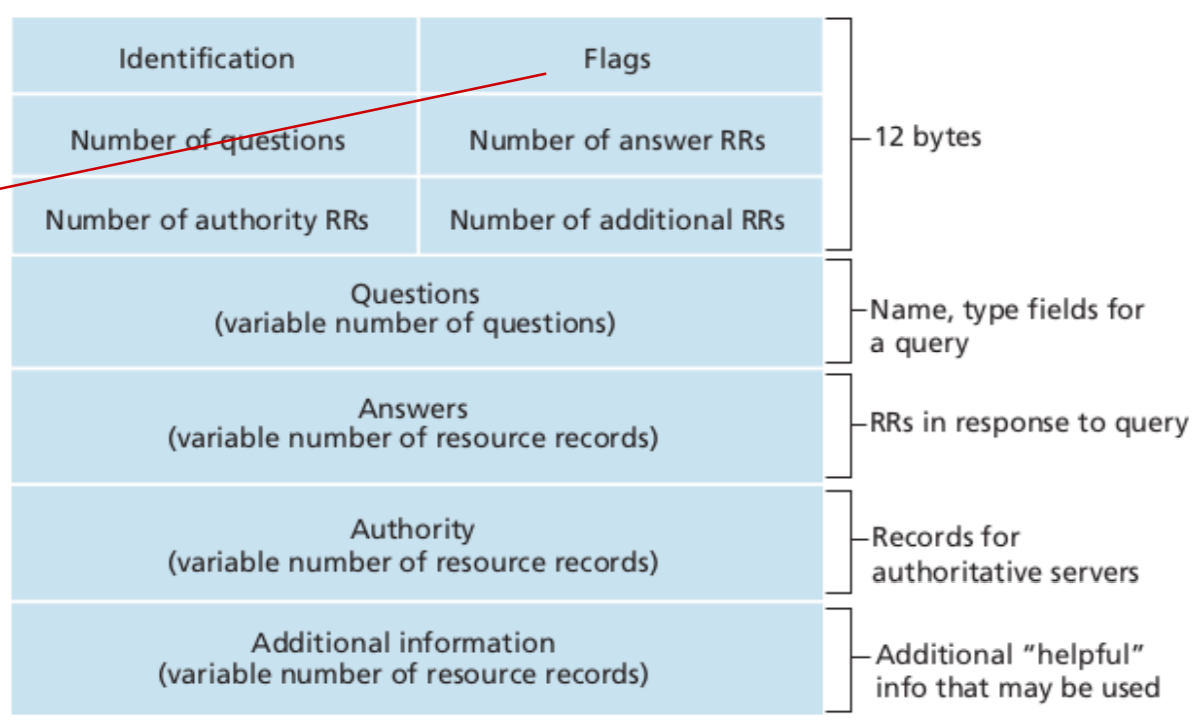
\includegraphics[width=12cm]{unit-17/figures/dns-message.png}
  \caption*{The general format of a DNS query or response message.}
\end{figure}

\subsubsection{DNS Registration}

When an organisation registers its host name \texttt{example.com} with a DNS registrar, the registrar inserts two RRs into the relevant TLD server.
These are a type~NS record for the name of the authoritative server of the organisation (\texttt{example.com}, \texttt{dns.example.com}, NS) and a type~A record for the IP address of the authoritative server (\texttt{dns.example.com}, \texttt{111.111.111.1}, A).
The authoritative server contains type~A records for its subdomains and a type~MX record for its mail server.


\end{document}
